%%%%%%%%%%%%%%%%%%%%%%%%%%%%%%%%%%%%%%%%%%%%%%%%%%%%%%%%%%%%%%%%%%%%%%%%
%    INSTITUTE OF PHYSICS PUBLISHING                                   %
%                                                                      %
%   `Preparing an article for publication in an Institute of Physics   %
%    Publishing journal using LaTeX'                                   %
%                                                                      %
%    LaTeX source code `ioplau2e.tex' used to generate `author         %
%    guidelines', the documentation explaining and demonstrating use   %
%    of the Institute of Physics Publishing LaTeX preprint files       %
%    `iopart.cls, iopart12.clo and iopart10.clo'.                      %
%                                                                      %
%    `ioplau2e.tex' itself uses LaTeX with `iopart.cls'                %
%                                                                      %
%%%%%%%%%%%%%%%%%%%%%%%%%%%%%%%%%%
%
%
% First we have a character check
%
% ! exclamation mark    " double quote  
% # hash                ` opening quote (grave)
% & ampersand           ' closing quote (acute)
% $ dollar              % percent       
% ( open parenthesis    ) close paren.  
% - hyphen              = equals sign
% | vertical bar        ~ tilde         
% @ at sign             _ underscore
% { open curly brace    } close curly   
% [ open square         ] close square bracket
% + plus sign           ; semi-colon    
% * asterisk            : colon
% < open angle bracket  > close angle   
% , comma               . full stop
% ? question mark       / forward slash 
% \ backslash           ^ circumflex
%
% ABCDEFGHIJKLMNOPQRSTUVWXYZ 
% abcdefghijklmnopqrstuvwxyz 
% 1234567890
%
%%%%%%%%%%%%%%%%%%%%%%%%%%%%%%%%%%%%%%%%%%%%%%%%%%%%%%%%%%%%%%%%%%%
%
\documentclass[12pt]{iopart}
\bibliographystyle{iopart-num_custom}
\usepackage{xcolor}
\usepackage{pifont}
\usepackage{comment}
\usepackage{acronym}
\usepackage{standalone}
\usepackage{academicons}
\usepackage{scalerel}
\usepackage{layouts}
%\usepackage{import}
\usepackage{subfig}
\usepackage{tikz}
\usetikzlibrary{decorations.pathreplacing,angles,quotes,shapes.geometric, arrows,calc}
\usetikzlibrary{svg.path}
\expandafter\let\csname equation*\endcsname\relax 
\expandafter\let\csname endequation*\endcsname\relax 
\usepackage{amsmath}
\usepackage{amssymb}
\usepackage{hyperref}
\usepackage[capitalize]{cleveref}

\usepackage[mathlines]{lineno}% Enable numbering of text and display math
\linenumbers\relax % Commence numbering lines


\newcommand{\gguide}{{\it Preparing graphics for IOP Publishing journals}}
%Uncomment next line if AMS fonts required
%\usepackage{iopams}  
\newcommand{\jordan}[1]{\textbf{\textcolor{red}{JORDAN: #1}}}
\newcommand{\siong}[1]{\textbf{\textcolor{blue}{SIONG: #1}}}
\newcommand{\chris}[1]{\textbf{\textcolor{green}{CHRIS: #1}}}
\newcommand{\michael}[1]{\textbf{\textcolor{orange}{MICHAEL: #1}}}
\newcommand{\dcc}{LIGO-PXXXXXXX}
%\input{tag.tex}
% Command for ORCID id's
\definecolor{orcidlogocol}{HTML}{A6CE39}
\tikzset{
  orcidlogo/.pic={
    \fill[orcidlogocol] svg{M256,128c0,70.7-57.3,128-128,128C57.3,256,0,198.7,0,128C0,57.3,57.3,0,128,0C198.7,0,256,57.3,256,128z};
    \fill[white] svg{M86.3,186.2H70.9V79.1h15.4v48.4V186.2z}
                 svg{M108.9,79.1h41.6c39.6,0,57,28.3,57,53.6c0,27.5-21.5,53.6-56.8,53.6h-41.8V79.1z M124.3,172.4h24.5c34.9,0,42.9-26.5,42.9-39.7c0-21.5-13.7-39.7-43.7-39.7h-23.7V172.4z}
                 svg{M88.7,56.8c0,5.5-4.5,10.1-10.1,10.1c-5.6,0-10.1-4.6-10.1-10.1c0-5.6,4.5-10.1,10.1-10.1C84.2,46.7,88.7,51.3,88.7,56.8z};
  }
}

\newcommand\orcidicon[1]{\href{https://orcid.org/#1}{\mbox{\scalerel*{
\begin{tikzpicture}[yscale=-1,transform shape]
\pic{orcidlogo};
\end{tikzpicture}
}{|}}}}

\usepackage{hyperref} %<--- Load after everything else

\begin{document}

\title{Generalised gravitational burst generation with Generative Adversarial Networks}

\author{
    J. McGinn \orcidicon{0000-0000-0000-0000},
    C. Messenger \orcidicon{0000-0001-7488-5022},
    I.S. Heng \orcidicon{0000-0000-0000-0000},
    M. J. Williams \orcidicon{0000-0003-2198-2974}
}

\address{University of Glasgow, Physics \& Astronomy Department, Glasgow G12 8QQ, UK}
%\ead{jordan.mcginn@glasgow.ac.uk}
\vspace{10pt}
%\begin{indented}
%\item[]\commitDATE\\\mbox{\small \commitID}\\\mbox{\dcc}
%\end{indented}

\begin{abstract}
The next generation of Gravitational wave detectors will accelerate the number
of ac{GW} detections such that we can gain new in site into the
physics behind the sources causing the phenomena. Numerical simulations and
matched filtering are the standard for detecting ac{GW}s for known
sources such as binary-black hole mergers. There are other sources of ac{GW}s
that remain elusive to standard modelling techniques and are expected to be
detectable. Here we construct a unmodelled burst generation scheme using
Generative adversarial networks - a powerful class of machine learning.
\chris{time to add a real abstract}
\end{abstract}

%
% Uncomment for keywords
%\vspace{2pc}
%\noindent{\it Keywords}: XXXXXX, YYYYYYYY, ZZZZZZZZZ
%
% Uncomment for Submitted to journal title message
%\submitto{\JPA}
%
% Uncomment if a separate title page is required
%\maketitle
% 
% For two-column output uncomment the next line and choose [10pt] rather than [12pt] in the \documentclass declaration
%\ioptwocol
%

\acrodef{GW}[GW]{gravitational wave}
\acrodef{CBC}[CBC]{compact binary coalescence} 
\acrodef{ML}[ML]{machine learning}
\acrodef{AI}[AI]{artificial intelligence}
\acrodef{CNN}[CNN]{convolutional neural network}
\acrodef{GAN}[GAN]{generative adversarial network}
\acrodef{CGAN}[CGAN]{conditional generative adversarial network}
\acrodef{ACGAN}[ACGAN]{auxilliary conditional generative adversarial network}
\acrodef{DCGAN}[DCGAN]{deep convolutional generative adversarial network}
\acrodef{CNN}[CNN]{convolutional neural networks}
\acrodef{BBH}[BBH]{binary black hole}

%%%%%%%%%%%%%%%%%%%%%%%%%%%%%%%%%%%%%%%%%%%%%%%%%%%%%%%%%%%%%%%%%%%%%%%%%%%%%%
%%%%%%%%%%%%%%%%%%%%%%%%%%%%%%%%%%%%%%%%%%%%%%%%%%%%%%%%%%%%%%%%%%%%%%%%%%%%%%
\section{Introduction}
%%%%%%%%%%%%%%%%%%%%%%%%%%%%%%%%%%%%%%%%%%%%%%%%%%%%%%%%%%%%%%%%%%%%%%%%%%%%%%
%%%%%%%%%%%%%%%%%%%%%%%%%%%%%%%%%%%%%%%%%%%%%%%%%%%%%%%%%%%%%%%%%%%%%%%%%%%%%%
%textwidth in inches: \printinunitsof{in}\prntlen{\textwidth}
\begin{comment}
\begin{itemize}
\item Need to introduce GWs - the current state of the field e.g. detections
and LVC papers \ding{51}
\item Introduce burst searches - what's the point of burst searches \ding{51} - lots of references 
\item Discuss the family of burst waveforms currently used and why - not in detail, just
an introduction \ding{51}
\item Introduce ML techniques in GWs \ding{51} - lots of references
\item What this paper does on GANs in 1 paragraph \ding{51}
\item Describe the structure of the paper 
\end{itemize}
\end{comment}

% introduce \ac{GW} astrophsyics
%
\ac{GW} astronomy is now an established field, starting with the first
detection of a binary black hole merger~\cite{Abbott2016} in September 2015.
Following this, the first and second observations runs (O1 and O2) of Advanced
LIGO and Advanced Virgo~\cite{Prospects-dets, AdvLIGO, AdvLIGO2, AdvVIRGO}
reported several more \ac{CBC} mergers~\cite{Abbott2016a, Abbott2017,
Abbott2017a, Abbott2017b}. On 17th August 2017 a binary neutron star merger was
observed alongside its electromagnetic counterpart for the first time, giving
rise to multi-messenger ac{GW} astronomy. 

% introduce burst searches
%
With these successes and continued upgrades to the detectors, further
detections of \acp{CBC} are expected to be commonplace in future advanced
detcetor observation runs. Another group of \ac{GW} signals that has thus far
been undetected is \ac{GW} ``bursts". \ac{GW} bursts are classed as transient
signals of typically short duration ($<$ 1s) whose waveforms are not accurately
modelled or are complex to reproduce. Astrophysical sources for such transients
include: Core collapse supernova~\cite{Fryer_2003}, Pulsar
glitches~\cite{Andersson_2001}, Neutron star post-mergers~\cite{Baiotti_2007}
and other as-yet unexplained astrophysical phenomena. 

% more details on burst searches
%
\ac{GW} searches for modelled signals so far have used a process called
matched-filtering,~\cite{Owen1998}, where a large template bank of possible
\ac{GW} waveforms are compared to the detector outputs. In order to increase
the chances of detection these template banks must span a large
multi-dimensional parameter space and the templates must be accurate, requiring
significant computational cost~\chris{the accuracy doesn't obviously lead to a
cost increase}. \ac{GW} bursts are un-modelled~\chris{except for the ones you
mentione before? SNe, glicthes, post-merger? }; therefore there are no
templates available and so matched-filtering is unsuitable for the detection of
these signals.  Instead, detection involves distinguishing the signal from
detector noise~\chris{but that's also what matched-filtering does}. Burst
searches look for excess power contained in the time-frequency
domain~\chris{all of them? In any case you have to provide references here to
the pipelines (cWB, x-pipeline, etc... Siong can help)} and rely on the
astrophysical burst waveform appearing in multiple detectors at similar times.
This is only possible if the detector noise is well characterised and the
candidate signal can be differentiated from systematic or environmental
glitches. 

% Discuss the family of burst waveforms currently used and why - not in detail, just
% an introduction 
%
\ac{GW} burst detection algorithms~\cite{Klimenko_2008, Aso_2008} are tested
and tuned using modelled waveforms that may or may not have astrophysical
significance but have easy to define parameters and share characteristics of
real bursts that are enough to simulate a \ac{GW} passing between
detectors~\chris{long sentence}. Such waveforms include sine-Gaussians: a
Gaussian modulated sine wave that is characterised by its central frequency and
decay parameter. Bandlimited white-noise bursts: white noise that is contained
within a certain frequency range and ring-downs which mimic the damped
oscillations after a \ac{CBC} merger.~\chris{seems strange to list only 3 of
the 5 that we will be using later on.}

% cut this text if not going to be used
%
\begin{comment}Such waveforms may have
long-duration, short bandwidth (ringdowns), long-duration, large bandwidth
(inspirals) and many algorithms make use of sine-Gaussians: a Gaussian
modulated sine wave that is characterised by it's central frequency and narrow
bandwidth.~\chris{not the time to try to describe the types of burst waveforms.
Also, be careful with satying things like ringdowns have narrow bandwidth. I
know we specify a single frequency but becuase of the short duration, the
signal is broad band. Look at the FFT} This makes it a great tool for
diagnosing LIGOs sensitivity to frequency.~\chris{strange unfinished sentence.} 
\end{comment}

% Introduce ML techniques in GWs
%
With the expectation that there will be many more \ac{GW} detections in the
future, there is a growing need for fast and efficient \ac{GW} analysis methods
to match the rising number of detections. While still in its infancy, \ac{ML}
applications to \ac{GW} analyses have already shown great potential for
overcoming data bottlenecks~\chris{what does that mean?}. \ac{GW} analysis in
areas of detection~\cite{Gabbard2017,Gebhard_2019,Krastev_2020}, glitch
classification~\cite{Bahaadini, George_2018,Razzano_2018} and parameter
estimation~\cite{gabbard2019bayesian, shen2019deterministic,
green2020gravitationalwave}~\chris{unfinished sentence, plus I wouldn't
reference the Shen paper}. Applying these algorithms show similar results to
matched-filtering techniques and have the benefit of being orders of magnitude
faster. \michael{We mention aspects related to detection (pattern matching) but
also metion PE in the same sentence and I think this is a bit
confusing.}~\chris{yes, the matched-filtering comp[arison is only relevent for
searches. The biggest speed gain is for the Bayesian PE. I also think that you
need to reference more of the ML-GW literature here. I've added Mervyn's SNe
paper, Joe's latest paper, our latest Gaussian ?Mixture model paper, 2 CW
papers and the recent ML review paper to the bibligrapohy file but there are
quite a few others. Have a look at the review to steal references. In each case
try to say 1 sentence about what they do if possible.}

% What this paper does on GANs in 1 paragraph - the point of the paper
%
In this work we aim to explore the use of \ac{ML} to generate and interpret
unmodelled \ac{GW} burst waveforms. Using the generative machine learning
model: \acp{GAN}, we train on five classes of known~\chris{are they known? In
what sense?} burst morphologies~\chris{fancy word - what about waveform class?}
in the time domain. Working with the assumption that \acp{GAN} construct smooth
$n$-dimensional vector spaces between their input and output, we can then
explore the space between the five classes to construct new
unmodelled~\chris{hybrid?} waveforms. As all the computationally expensive
processes occur during training, the learned model after training is able to
produce waveforms in fractions of a second and in fact produce waveforms that
are impossible~\chris{never say never (or impossible)} to produce with current
techniques. These new varieties of waveforms can then be used to diagnose
detection algorithms and gain new insight into sources of \ac{GW}
bursts~\chris{yes, they can help diagnose or calibrate or assess the sensitivty
of detection algorithms but also allow us to better train our algorithms to a
broader range of possible signals and therefore enhance our detection ability}. 

% the structure of the paper
%
This paper is organised as follows: \jordan{unstructured at the
moment}~\chris{time to add the structure.}

%%%%%%%%%%%%%%%%%%%%%%%%%%%%%%%%%%%%%%%%%%%%%%%%%%%%%%%%%%%%%%%%%%%%%%%%%%%%%%
%%%%%%%%%%%%%%%%%%%%%%%%%%%%%%%%%%%%%%%%%%%%%%%%%%%%%%%%%%%%%%%%%%%%%%%%%%%%%%
\section{Generative Adversarial Networks}
%%%%%%%%%%%%%%%%%%%%%%%%%%%%%%%%%%%%%%%%%%%%%%%%%%%%%%%%%%%%%%%%%%%%%%%%%%%%%%
%%%%%%%%%%%%%%%%%%%%%%%%%%%%%%%%%%%%%%%%%%%%%%%%%%%%%%%%%%%%%%%%%%%%%%%%%%%%%%

\begin{comment}
\begin{itemize}
\item Describe GANs in detail but really focus on the fact that the reader is a
GW data analyst - not a computer scientist \ding{51}
\item A diagram would be very useful \ding{51}
\item Do not discuss our specific case here - just stay general \ding{51}
\item A subsection on the specific advanced flavour of GAN that you are using
here - motivate this choice. \ding{51}
\end{itemize}
\end{comment}

% introduce GANs
%
\subsection{Artificial neural networks}

\begin{figure}
    \begin{minipage}[b]{0.3\linewidth}
        \subfloat[]{\label{fig:perceptron}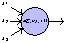
\includegraphics[width=\linewidth,height=0.65\linewidth]{figures/neural_network-figure0.pdf}}
        \par
        \vspace{\baselineskip}
        \subfloat[]{\label{fig:tanh_activation}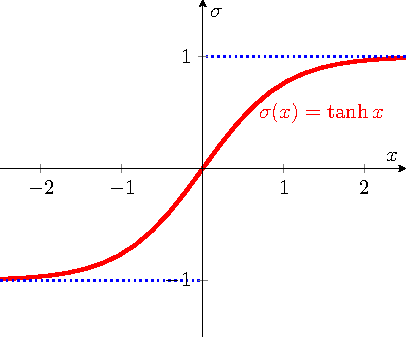
\includegraphics[width=\linewidth,height=0.65\linewidth]{figures/neural_network-figure1.pdf}}
    \end{minipage}
        \begin{minipage}[b]{0.7\linewidth}
        \subfloat[]{\label{fig:neural_network}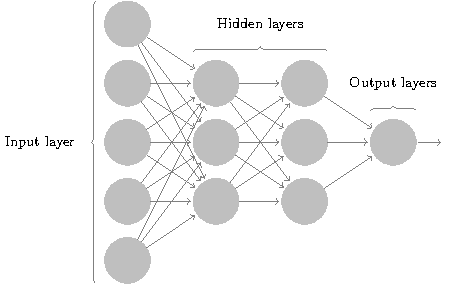
\includegraphics[width=\linewidth,height=0.65\linewidth]{figures/neural_network-figure2.pdf}}
    \end{minipage}
    \caption{Neural Networks (a) A single neuron taking a vector of inputs and
returning a single output based on the weights, bias and activation function
of the network. (b) The hyperbolic tangent used as an activation
function.~\chris{is this the actual activation that you use in the GAN?
otherwise why focus on it alone, you could plot a handful on the same plot} (c)
A fully connected~\chris{you haven't mentioned what a fully connected network
actually is in the text} neural network containing two hidden layers that performs a
mapping of an input vector to a single output. \michael{Equation in the
neuron looks very small}~\chris{I agree, but the equation in (b) is even
smaller. I would also recommed that you make the style of the FC network hidden
and output layer neurons the same as the single perceptron in terms of colours.
You could put $x_i$s in the input layer.}}
\end{figure}

% inroduce the concept of ML
%
Since the birth of programmable computers, people have wondered if machines can
develop true intelligence beyond formal mathematical procedures. Today, \ac{ML}
aims to learn apparent relationships held within the given data or `training
data' in order to make accurate predictions without the need for additional
programming. A common approach in \ac{ML} relies on the computer learning on
past experience to make decisions on future events. \michael{Not sure about the
use of computer here, maybe \textit{relies on a model}?} The hierarchical
nature of this approach means that the machine can build complicated concepts
from simpler ones~\chris{what hierarchical nature? You haven't mentioned
anything about that.}. This branch of \ac{AI} is called deep
learning~\chris{OK, but as long as you explain the hierarchy thing and how it
implies complicated concepts from simpler ones.}. 

% Introduce basic neural networks - a perceptron layer
%
Neural networks are the quintessential~\chris{really? quintessential?} \ac{ML}
algorithm that aims to approximate a function. They are built from many single
processing units called neurons. The simpliest Neural Network is the perceptron
layer~\cref{fig:perceptron} which holds a single neuron that takes several real
inputs $x_{1},\ldots, x_{i}$~\chris{and outputs what? also $i$ is the index and not the "final" index}
and maps them to an output according to the linear equation 
%
\begin{align}
\sigma(\sum_i w_i x_i + b),
\label{eqn:neuron}
\end{align}
%
\chris{it's not an equation if it's not equal to something. Please make it
eaqual something.} where $w$ and $b$ are the weights and bias and $\sigma$
denotes the activation function. The weights are numbers which can be thought
as the strength between connections~\chris{what connestions? between what
objects?}. The output of a neuron is called its activation and different
choices of activation function allow the user~\chris{are we users or developers
or what?} to simulate various models. A common example of an activation
function is the hyperbolic tangent~\cref{fig:tanh_activation} that is used when
the outputs of the network must be both positive and negative~\chris{how can an
output be both positive and negative. The language is ambiguous and confusing}
and re-scaled to $[-1,1]$~\chris{at this stage in the explanation the reader
has no idea what an output would look like or why it would be rescaled}. It is
often useful to introduce a bias, $b$, such that the neuron remains inactive
above zero but is active when the sum reaches a defined threshold. This bias is
added before the activation function and it tells us how high the weighted sum
needs to be before the neuron becomes active.~\chris{well kind of, but also not
really. I would advise you to rewrite this (if we keep it) in a minimalist
style just explaining what each item is and not trying to describe what it
does.}

% the cost or loss function
%
The output of a single neuron is defined by~\cref{eqn:neuron} and gives a
prediction $\hat{y}$ that can be compared to the real value $y$~\chris{what the
hell is $y$, it's not been mentioned before} through a loss (also known as a
cost) function. If the loss is non-zero~\chris{no, it doesn't matter whether
the number is above or below or equal to zero, the machine will try to minimise
the number (if negative, it will try to make it more negative)}, the network
must work to minimise this function by updating the weights in the negative
direction of the loss gradient in a process referred to as gradient
descent~\chris{give reference and also make the distinction between this and
the actual method used to do it, back progagation}. This loss function plays a
critical role in how neural networks learn~\chris{OK, but are you going to
expand on that or just leave it there? As far as I can tell from the text it's
the *only* way network's learn so that's pretty critical and already evident}.

% basic network structure
%
A neural network contains many single neurons connected in a layered structure
as shown in~\cref{fig:neural_network}. The activations of the first layer (or
input layer) act as the inputs to the second layer and so on until the output
layer. Multi-layered neural networks have intermediate layers between the input
and output stages dubbed the hidden layers as the computations performed are
not accessible to the user~\chris{well that's not really true. We can access
everything if we want but it depends on what you define as a user. Best to
simply state what they're clalled and no need to give a reason.}. The network
can be thought of as a function F: $\mathbb{R}^N\rightarrow
\mathbb{R}^M$~\chris{does F not have to be in math-mode too? Is is a
mathematical symbol?} reliant on how activations from one layer bring
activations in the next~\chris{yes, kind of, but also reliant on the trained
weights and biases too, so actually reliant on everything}. The system is
analogous to biology, where, some groups of neurons in animal brains cause
certain others to fire~\chris{best to stay away from analogies like these where
the practical specifics can be picked apart}. 

%%%%%%%%%%%%%%%%%%%%%%%%%%%%%%%%%%%%%%%%%%%%%%%%%%%%%%%%%%%%%%%%%%%%%%%%%%%%%%
\subsection{Convolutional Neural Networks}
%%%%%%%%%%%%%%%%%%%%%%%%%%%%%%%%%%%%%%%%%%%%%%%%%%%%%%%%%%%%%%%%%%%%%%%%%%%%%%
%
\acp{CNN} are designed to work with grid-like input structures that exhibit
strong local spatial dependencies. An example would be a two-dimensional image
as each coloured pixel has similar intensities to their near
neighbours~\chris{it's not about that really, it's like you said, it's about
spatial relationships}. The value contained in each pixel can be thought of as
adding an additional dimension or channel to the image~\chris{no, the dimension
and channel are specifically defined. A 2D image has 2 dimensions. An RGB image
has 3 numbers per pixel and these are typcally stored as channels. Channels are
dealt with differently to dimensions}. Although most work with \acp{CNN}
involve image-based data, they can be applied to other spatially adjacent data
types such as time-series and text items. \acp{CNN} are defined by the use of a
convolution operation, a mathematical operation that expresses the amount
overlap between functions. The convolution is applied by shifting one grid-like
structure over the other, drawing out spatially important features between the
two~\chris{yes, but what is being dragged over what? Time to define the
convolutional neuron? Maybe add an equation?}. A strided convolution reduces
the dimensionality of the input while retaining spatial features \michael{How?
This is core part of the architecture of the GAN but is quite vague, I don't
think it's obvious that stride imples moving the filter further. Maybe
something like: \textit{the distance by which the grid is shifted is known as
the stride and increasing it reduces the dimensionality of the
output}}~\chris{why are we talking about strides at this point? Are they
important for the GAN? You haven't mentioned kernel sizes or dropout. are these
equally important?}. This can result in a loss of information along the
borders~\chris{the borders of what?}. To combat this, the input is padded with
zeros at the edges which does not interfere with the convolutional operation.
The output of the convolutional layer is then passed to an activation function.

~\chris{I'm getting the sense that these 2 sections of ANNs and CNNs aren't
really helpful in their current state. They should either be removed OR tidied
up. I don't think they need to be expanded upon but various statements can be
removed and other important things can be added. Imagine reading this with no
knowledge of ML. Do you get informed by this or confused?} 

%%%%%%%%%%%%%%%%%%%%%%%%%%%%%%%%%%%%%%%%%%%%%%%%%%%%%%%%%%%%%%%%%%%%%%%%%%%%%%
\subsection{GANs}
%%%%%%%%%%%%%%%%%%%%%%%%%%%%%%%%%%%%%%%%%%%%%%%%%%%%%%%%%%%%%%%%%%%%%%%%%%%%%%
%
% basic intro to GANs
%
A subset of deep learning that has seen fruitful development in recent years
are \acp{GAN}~\cite{Goodfellow2014}. These unsupervised~\chris{they have
training data don't they? Is that unsupervised?} algorithms learn patterns in a
given training data set using an adversarial process. The generations from
\acp{GAN} are state-of-the-art~\chris{a phrase that will not stand the test of
time} in fields such as high quality image
fidelity~\cite{brock2018large,karras2019analyzing}, text-to-image
translation~\cite{reed2016generative}, and video
prediction~\cite{liang2017dual} as well as time series
generations~\cite{esteban2017realvalued}~\chris{do we still not have any other
GW GAN applications to reference or are we hoping to still be the first?}. 

% Basic components of a GAN
%
\acp{GAN} train two competing neural networks, consisting of a discriminator
network that is set up to distinguish between real and fake data and a
generator network that produces synthetic (fake) versions of the real data.
\michael{Is it clear to the reader that the \textit{fake} data is the same as
the synthetic data?} The generator performs a mapping from an input noise
vector $\mathbf{z}$, that is usually sampled from a $n$-dimensional~\chris{be
careful with statments about $n$-dimensions since $n$ is a variable and could
mean the number of latent dimensions or the number of class dimensions or data
dimensions, etc...} Gaussian space known as the latent space, to its
representation of the data, and the discriminator maps its input $\mathbf{x}$ to
a probability that the input came from either the training (real) data or
generator (fake). 

% training a GAN
%
During training, the discriminator is given a batch~\chris{you have not
introduced batches yet. Best to do that in the ANN section} of samples that
contains one half real data and one half fake data which it then makes
predictions on.  The loss for the discriminator is calculated by comparing its
predictions to the labelled data through the binary cross-entropy function.
\jordan{note to myself: This is important since eqn 2 is derived from it (thats
where the logs come from)}~\chris{either give a reference to binary cross
entropy or define it here mathematically}. The training process of a \ac{GAN}
alternatively updates the weights of the discriminator and generator based on
information on its competitors loss function~\chris{you haven't fully explained
how the loss is computed in the 2 phases of each training pass. I recommend
that you add that here other wise discussion of generator loss and discrimator
loss makes no sense.}. This loss of the discriminator is used to update the
weights of the generator to produce more realistic samples of the input
distribution, the loss of the generator encourages the discriminator to update
its classification abilities. \acp{GAN} seek to find an equilibrium between the
generator and discriminator in the form of a two-player game that can be
summarised by 
%
\begin{align}
  \mathop{\text{min}}_{G}  \mathop{\text{max}}_{D} V(D,G) &= \mathbb{E}_{\mathbf{x} \sim p_{\text{r}}(\mathbf{x})} [\text{log} D(\mathbf{x})] + \mathbb{E}_{\mathbf{z} \sim p_{\text{z}}(\mathbf{z})} [\text{log}(1-D(G(\mathbf{z})))],
\label{equation:GANloss}
\end{align}
%
% remove these comments 
%
\begin{comment}
Both networks compete in
a minimax game~\chris{what is a minimax game? references?} which the generator
is trying to minimise and the discriminator is trying to
maximise:~\chris{nicely written, however, it needs an extra 25\% explanation
for people not familar with ML or GANs in particular. Try to spell things out
more. Also refer to Fig 1 somewhere in this section.}
\end{comment}
%
where $V$ is an objective function that is to be optimised. Objective functions
are a general term for either a loss function (to be minimized) or a negative
loss function (to be maximised). We use $D$ to define the discriminator
function~\chris{output interpreted as a probability?} , $G$ for the generator
function and ${\mathbf{x} \sim p_{\text{r}}(\mathbf{x})}$, ${\mathbf{z} \sim
p_{\text{z}}(\mathbf{z})}$ are samples taken from the training data and
generated data respectfully~\chris{no, $z$ can't be from the data since it's
not called $x$. It is from the latent space distribution.}. In practice this
approach was found to be unstable \michael{Cite?}~\chris{unstable for us or
unstable in general, also add reference.}. Early on in training the generators
weights are initialised randomly meaning that the early generations are noisy
and uninformative. This means that the discriminator can easily learn to spot
the fake generations and so the discriminator wins and the generator cannot
continue to improve. To overcome this the framing~\chris{what is framing in
this context?} of the generator is often changed. Rather than minimizing
$\text{log}(1-D(G(\mathbf{z})))$ the objective now is to maximise
$\text{log}(D(G(\mathbf{z})))$, that is, to maximise the probability of the
generations being predicted as real. The idea being that we always want the
losing side to be able to leverage \michael{information?} from its
competitor.~\chris{OK, does this all mean that the previous equation is wrong?
If so, why quote it. Just use the actual correct equation and explain why it's
correct rather than explaining why something is wrong. I would also try to link
up this equation with how we actually train i.e., we compute the first term by
drawing samples from the training set $x$ and getting the average log-prob of
the discriminator (not quite true since we actually input a mix of real $x$ and
fake $G(z)\rightarrow x'$). Then we take a set of fake $x'$ made using $G(z)$
with $z$ drawn from the latent space, and get the loss (but we switch the
labels hence the $1-D(G(z))$. See what I mean? You shouls also refer to Fig 2
here.} 
%

% describing the problems with GANs 
%
In theory, the adversarial process will eventually lead to the local Nash
equilibrium~\cite{Nash1950} whereby both neural networks are trained
optimally~\chris{vague and not informative statement. What does optimal mean
here?}. In practice, however, \acp{GAN} are notoriously difficult to train with
difficulties that include: Non-convergence, where the model parameters
oscillate and the loss never converges, mode collapse where the generator
produces a limited diversity of samples, and diminishing gradients when
applying gradient descent to a loss function that is discontinuous.~\chris{OK,
difficult to train. I understand. Why are you telling the reader this? Will we
be referring back to these issues later?}

%%%%%%%%%%%%%%%%%%%%%%%%%%%%%%%%%%%%%%%%%%%%%%%%%%%%%%%%%%%%%%%%%%%%%%%%%%%%%%
\subsection{Conditional GANs}
%%%%%%%%%%%%%%%%%%%%%%%%%%%%%%%%%%%%%%%%%%%%%%%%%%%%%%%%%%%%%%%%%%%%%%%%%%%%%%

% introduce CGANs and ACGANs
%
To gain more control over what a GAN is able to generate, a conditional variant
of \acp{GAN} named \acp{CGAN}~\cite{cgan} was introduced by feeding in extra
information into the generator and discriminator such as a class label or
attribute label, $c$. The objective function~\cref{equation:GANloss}~\chris{I
think it owuld be be best if you just stick to loss function rather than
switching between loss and objective} is then
%
\begin{align}
  \mathop{\text{min}}_{G}  \mathop{\text{max}}_{D} V(D,G) &= \mathbb{E}_{\mathbf{x,c} \sim p_{\text{r}}(\mathbf{x,c})} [\text{log} D(\mathbf{x,c})] + \mathbb{E}_{\mathbf{z} \sim p_{\text{z}}(\mathbf{z}),\mathbf{c} \sim p_{\text{r}}(\mathbf{c})} [\text{log}(1-D(G(\mathbf{z,c})))].
\label{equation:cGANloss}
\end{align}

This simple addition has shown to work well in practice, for instance in
image-to-image translation~\cite{isola2016imagetoimage}. We will be using a
conditional GAN for this study.~\chris{OK, but you have not defined the new
changes to the loss function in the text. Please indicate that the training
data and labels are being drawn from a joint distribution $p_r(x,c)$ and when
making fake data you are drawing from $p_r(c)$ independent of =$p(z)$. However,
what does the $r$ stand for and why is it important, and what defines $p_r(c)$?}

~\chris{Finally, you need to refer to and discuss Figure 2. It is currently
neither referenced or discussed.}

% get rid of these comments if they are no longer useful
%
\begin{comment}adds structure to the latent space by providing the
generator with a class or attribute label. The generator learns to segment the
latent space by clustering distributions which have similar properties, making
a point in latent space conditional on a class~\chris{are we sure about this?
all classes share the same latent space and I don't think that the space gets
segmented into areas corresponding to different classes - I do think that it
gets broken down into spaces with different intrinsic physical properties e.g.,
high frequency, long duration, etc...}.
\end{comment}
%
\begin{comment}
This idea was extended further with
\acp{ACGAN}~\cite{odena2016conditional} that require the discriminator to
output a probability of data belonging to each class. A pictorial
representation on the differences between these approaches is shown in
Fig.~\ref{fig:gan_comparison} \jordan{self note: Probably move away from ACGAN part, standalone aux classifiers can be trained later if that's what you want}. 
\end{comment}

\begin{figure}
    \centering
        %\documentclass{article}
%\usepackage{comment}
%\usepackage{tikz}
%\usetikzlibrary{shapes.geometric, arrows, calc}

%\begin{document}
    
\begin{tikzpicture}[node distance=2cm]

\tikzstyle{zinput} = [rectangle, rounded corners, text centered, draw=black]%, fill=red!30]
\tikzstyle{generator} = [rectangle, rounded corners, text centered, draw=black]%, fill=red!30]
\tikzstyle{X real} = [rectangle, rounded corners, text centered, draw=black]%, fill=red!30]
\tikzstyle{X fake} = [rectangle, rounded corners, text centered, draw=black]%, fill=red!30]
\tikzstyle{X real} = [rectangle, rounded corners, text centered, draw=black]%, fill=red!30]
\tikzstyle{discriminator} = [rectangle, rounded corners, text centered, draw=black]%, fill=red!30]
\tikzstyle{real/fake} = [rectangle, rounded corners, text centered, draw=black]%, fill=red!30]

\tikzstyle{arrow} = [thick,->,>=stealth]

\node (r) [X real] {\textbf{X} real};
\node (f) [X fake, right of = r] {\textbf{X} fake};
\node (G) [generator,above of = f, scale = 2] {\textbf{G}};
\node (z) [zinput] [zinput, above of = G] {\textbf{z} (noise)};
\node (D) [discriminator, below of = f, xshift = -1cm, scale = 2] {\textbf{D}};
\node (rf) [real/fake, below of = D] {real/fake};

\draw [arrow] (z) -- (G);
\draw [arrow] (G) -- (f);
\draw [arrow] (r) edge[out=270,in=90] (D);
\draw [arrow] (f) edge[out=270,in=90] (D);
\draw [arrow] (D) -- (rf);

\end{tikzpicture}
%\end{document}
%     without .tex extension
        \begin{tikzpicture}[node distance=2cm]

\tikzstyle{zinput} = [rectangle, rounded corners, text centered, draw=black]%, fill=red!30]
\tikzstyle{generator} = [rectangle, rounded corners, text centered, draw=black]%, fill=red!30]
\tikzstyle{X real} = [rectangle, rounded corners, text centered, draw=black]%, fill=red!30]
\tikzstyle{X fake} = [rectangle, rounded corners, text centered, draw=black]%, fill=red!30]
\tikzstyle{X real} = [rectangle, rounded corners, text centered, draw=black]%, fill=red!30]
\tikzstyle{discriminator} = [rectangle, rounded corners, text centered, draw=black]%, fill=red!30]
\tikzstyle{real/fake} = [rectangle, rounded corners, text centered, draw=black]%, fill=red!30]
\tikzstyle{coutput} = [rectangle, rounded corners, text centered, draw=black]%, fill=red!30]

\tikzstyle{arrow} = [thick,->,>=stealth]

\node (r) [X real] {\textbf{X} real};
\node (f) [X fake, right of = r, xshift = 0cm] {\textbf{X} fake};
\node (G) [generator,above of = f, scale = 2] {\textbf{G}};
\node (z) [zinput] [zinput, above of = G, xshift = 1cm] {\textbf{z} (noise)};
\node (c) [coutput, left of = z] {\textbf{c} (class)};
\node (D) [discriminator, below of = f, xshift = -1cm, scale = 2] {\textbf{D}};
\node (rf) [real/fake, below of = D] {real/fake};
%\node (co) [coutput, left of = rf, xshift = -0.5cm] {c = 1, 2, ...};

\draw [arrow] (z) edge[out=270,in=90] (G);
\draw [arrow] (c) edge[out=270,in=90] (D);
\draw [arrow] (c) edge[out=270,in=90] (G);
\draw [arrow] (c) edge[out=270,in=90] (r);
\draw [arrow] (G) -- (f);
\draw [arrow] (r) edge[out=270,in=90] (D);
\draw [arrow] (f) edge[out=270,in=90] (D);
\draw [arrow] (D) edge[out=270,in=90] (rf);
%\draw [arrow] (D) edge[out=270,in=90] (co);

\end{tikzpicture}%     without .tex extension
    \caption{Comparison of the original GAN method and the
Conditional-GAN method. For CGANs the training data requires a label denoting
its class that is also fed to the generator which then learns to generate
waveforms based on the input label.~\chris{OK, a few things. Try to separate
these a bit and maybe make them subplots with sublabels indicating GAN and CGAN
distinction. Replace noise with latent (or otherwise). Noise implies GW data
noise which it is not. Overall it's a bit basic and doesn't indicate either the
2 competing training steps or any aspect of the loss or specify that $x$ and
$z$ (and $c$) are drawn from distributions already defined in the text. Maybe it's OK without
that. As for the CGAN, I'm troubled by the fact that there is only one $c$ box.
It implies that the same $c$ value is given to each real and fake $x$ data when
in fact each $x$ sample has it's own randomly drawn $c$ value.}} \label{fig:gan_comparison}
\end{figure}

%%%%%%%%%%%%%%%%%%%%%%%%%%%%%%%%%%%%%%%%%%%%%%%%%%%%%%%%%%%%%%%%%%%%%%%%%%%%%%
%%%%%%%%%%%%%%%%%%%%%%%%%%%%%%%%%%%%%%%%%%%%%%%%%%%%%%%%%%%%%%%%%%%%%%%%%%%%%%
\section{Methodology}
%%%%%%%%%%%%%%%%%%%%%%%%%%%%%%%%%%%%%%%%%%%%%%%%%%%%%%%%%%%%%%%%%%%%%%%%%%%%%%
%%%%%%%%%%%%%%%%%%%%%%%%%%%%%%%%%%%%%%%%%%%%%%%%%%%%%%%%%%%%%%%%%%%%%%%%%%%%%%

\begin{comment}
\begin{itemize}
\item Need to introduce the scheme you propose to use
\item A paragraph or subsection on the data generation being very clear on all
5 waveform models and the prior parameter space for each \ding{51}
\item A subsection on the design of the network architecture \ding{51}
\item A subsection on the "box" and why we implement it \ding{51}
\item A subsection on the training of the network - give rough timings and rule
of thumb decisions made
\item Do not discuss the results here 
\end{itemize}
\end{comment}

% introduce the training data
%

\begin{table}[hb]
\centering
\caption{Burst training parameters~\chris{Add a bit more caption description
here. Plus address the issues of the actual distributions used (uniform) and
how you include the BBH parameters. It's also not obvious that all the classes
share the same 3 parameters.}}
%\footnotesize
\begin{tabular}{@{} l l l l l l }
\br
\hline
 Waveform & Central frequency  & Decay & Central time epoch & Mass range \\
 & (Hz) & (s) & (s) & ($\textrm{M}_{\odot}$) \\
\mr
Sine-Gaussian & 70 - 250 & 0.004 - 0.03 & 0.4 - 0.6 & N/A  \\  
Ringdown & 70 - 250 & 0.004 - 0.03 & 0.4 - 0.6 & N/A \\
White-noise burst & 70 - 250 & 0.004 - 0.03 & 0.4 - 0.6 & N/A  \\
Gaussian pulse & N/A & 0.004 - 0.03 & 0.4 - 0.6 & N/A  \\
BBH & N/A & N/A & N/A & 5 - 70  \\
 \br
\end{tabular}\\
\label{Tab:training_parms}
\end{table}
\normalsize

% introduce the signal models
%
\ac{GW} burst signals remain an unmodelled phenomenon~\chris{as in the
introduction I think you need to make the distinction between unmodelled and
modelled burst analyses}, as such, current detection algorithms exploit the
fact that astrophysical signals will appear within data from multiple detectors
in coincidence and share the same waveform morphology.~\chris{I have added to
this first sentence but it still doesn't naturally lead intpo the next one} We
propose a signal generation scheme using a \ac{CGAN} trained on burst-like
waveforms. We call this \texttt{BurstGAN}~\chris{give reference to code repo
here} and is a \ac{CGAN} trained on five signal classes each spanning a range
of prior signal parameters. The signal classes are:

% list the 5 waveform classes
%
\begin{itemize}
%
\item {\bf Sine-Gaussian}: $h_{\text{sg}}(t) = A \exp\left[ - (t-t_{0})^2 /
\tau^2 \right] \sin (2 \pi f_0 (t-t_0))$, a sinusoidal wave with a Gaussian
envelope characterised by a central frequency, $f_0$.~\chris{what about
amplitude, time of arrival and initial phase? For all the other classes too.}
%
\item {\bf Ring-down}: $h_{\text{rd}}(t) = A \exp \left[-{(t-t_0)} / {\tau}
\right] \sin(2 \pi f_0 (t-t_0))$, with frequency $f_0$ and duration $\tau$
%
\item {\bf White-noise bursts}: $h_{\text{wn}}(t_j) = Ag_j\exp\left[ -
(t-t_{0})^2 / \tau^2 \right]$ where $g_j$ are drawn from a zero mean unit
variance Gaussian distribution and ahave a bounded frequency bandwidth $\Delta
f$ and duration $\tau$~\chris{no, they have a Gaussian envelope with a duration
parameter $tau$, we don't explicitly define the bandwidth}.
%
\item {\bf Gaussian pulse}: $h_{\text{gp}}(t) = \exp(-t^2 / \tau^2)$ with
duration parameter $\tau$.
%
\item {\bf Binary-black hole}: Simulated using the IMRPhenomD
waveform~\cite{Khan_2016} routine from LALSuite~\cite{lalsuite} which models
the inspiral, merger and ringdown of a \ac{BBH} waveform. The component masses
lie in the range of [5,70] $\textrm{M}_{\odot}$ with zero spins and we fix
$m_1>m_2$. The mass distribution is approximated by a power law with
index of 1.6~\cite{Abbott_2019}. The signals are generated using random right
ascensions and declinations uniform over the sky and the inclinations are drawn
from the cosine of a uniform distribution in the range [-1,1].~\chris{OK, we
have an issue here. First the prior parameters and ranges are being defined
here rather than in the table with the other classes. Second, you are
randomising the sky in order to get random antenna patterns which only act to
change the relative amplitudes in multiple detectors - whcih we don't use any
more. So I would say that you shoudl only use the plus polarisation since it is
the same as the cross but pi/2 out of phase.}  
%
\end{itemize}
%
The location of the peak amplitude of the waveforms (corresponding to the
mid-points of all but the ring-down and \ac{BBH} classes) are randomly drawn to
be within [0.4, 0.6] sec from the start of the 1 sec time interval and all
training waveforms are sampled at 1024 Hz.  The parameter prior ranges are
defined in~\cref{Tab:training_parms}.~\chris{Yes, those are the ranges but what
are the distributions?}

%%%%%%%%%%%%%%%%%%%%%%%%%%%%%%%%%%%%%%%%%%%%%%%%%%%%%%%%%%%%%%%%%%%%%%%%%%%%%%
\subsection{Architecture details}
%%%%%%%%%%%%%%%%%%%%%%%%%%%%%%%%%%%%%%%%%%%%%%%%%%%%%%%%%%%%%%%%%%%%%%%%%%%%%%
%
% Introduce some architecture features
%
Extensions to the original \ac{GAN} method such as the
\ac{DCGAN}~\cite{Radford2015} have been widely praised for enabling a stable
\ac{GAN} architecture. Most GANs now replace fully connected layers, where each
neuron is connect to all the neurons in the previous and next layer, with
convolutional layers. \acp{CNN}~\michael{capitalisation, not sure how it works
with the accronyms package}~\chris{I will fix this} are designed to work with
grid-like structures with close local dependencies like image and text based
data, however, there are examples of audio synthesis
work~\cite{DBLP:journals/corr/abs-1809-11096}.~\chris{this text sounds very
similar to the CNN text from earlier. Do you need this here? Can you simply say
that we are using a DCGAN architecture or say that our networks use
convolutional layers and then move on?}

% specifically define our architecture
%
We adopt the suggestions
of~\cite{Radford2015,DBLP:journals/corr/abs-1809-11096}, lengthening
one-dimensional convolution kernels on both the generator and
discriminator~\chris{what does this statment actually mean and why are you
opening the paragrpah with it?}.  The Generator model is fully convolutional,
upsampled using strided transposed~\chris{you mentioned strides before but not
transposing. Can you explain that aspect seomwhere earlier on.} convolutions
with batch normalisation~\chris{same here, can you mention it earlier} in the
first layer and ReLU~\chris{you can easily mention ReLU and other activations
earlier} activations throughout with the exception of the Tanh activation for
the output layer~\chris{why do you need this for the output? State that it is
to guarantee the output function is bound between [-1,1]}. Each transposed
convolutional layer uses a kernel size of $18\times 1$~\chris{by saying 18x1
you are saying that you are using a 2D kernel with width 1 but why not just say
you use a 1D kernel of size 18?} and stride of 2. The discriminator network
mirrors that of the generator without batch normalization~\chris{why?}, using
LeakyReLU activations, SpatialDropout, and a 2-stride convolution for
downsampling~\chris{any reason for these choices?}. The discriminator output is
a single node with Sigmoid activation that can be interpreted as a probability
of the the signal being real. This model is trained with binary cross
entropy~\chris{how exactly if the output is 1 number rather than 2 (binary)?}.
The full architecture description can be seen in~\cref{Tab:hyperparameters}.
~\jordan{still too technical im not sure if we need to go into more detail on
each thing mentioned.} \michael{This para doesn't seem to technical to
me}~\chris{same here, not too technical but lacking detail and motivation for
choices.}
%~\chris{OK, very technically tight but too computer sciencey. Try to make it
%human readbale for a physicist and refer to the table of parameters in the
%appendix.}

% describe the hyperparameter tunings
%
Neural networks and subsequently \acp{GAN} have multiple parameters a developer
can tune when designing the model and these are referred to as hyperparameters.
The final network design used in this work comes from the use of trial and
error and the initial designs influenced by the available literature. We found
that the \ac{GAN} performed better with both networks having the same number of
layers and neurons which should~\chris{should? well does it?} encourage even
competition between the generator and discriminator.  After tuning the multiple
hyperparameters (see \cref{Tab:hyperparameters}), the \ac{GAN} was trained on
$10^5$ signals which contained an even mixture~\chris{be a bit more specific
about what an even mixture is - technically they are drawn from a categorical
distribution with equal propabilities for each class} of
sine-Gaussian~\chris{Gauss was a person so we have to capitalise his stuff},
ring-down, white noise bursts, Gaussian pulse and \acp{BBH} for 1000 epochs and
takes $\Or$(2) days to train~\chris{on what? be specific}. A larger batch size
saw a small increase in performance~\chris{what is performance in this case} at
the cost of training speed and we decided that 128~\chris{128 what? Also, why
pick on batch size as the thing to comment on here? What about learning rate,
kernel size, etc...} was a fair compromise. 

\begin{comment}
include Plot_NN to show generator architecture
\end{comment}

~\chris{Please add a loss plot and use a paragrpah to describe what is going
on.}

%%%%%%%%%%%%%%%%%%%%%%%%%%%%%%%%%%%%%%%%%%%%%%%%%%%%%%%%%%%%%%%%%%%%%%%%%%%%%%
\section{Results}
%%%%%%%%%%%%%%%%%%%%%%%%%%%%%%%%%%%%%%%%%%%%%%%%%%%%%%%%%%%%%%%%%%%%%%%%%%%%%%


\begin{comment}

\begin{itemize}
\item Begin by outlining the type of results you will be presenting
\item A subsection on the general quality of generated waveforms - we may need
to have overlaps between generated wavefoms and training data (maybe)
\item A subsection on the descriminator - maybe a confusion matrix?
\item a subsection on the latent space varaition within each class - fixed
class, sliding in latent space.
\item A subsection on the class space variation - fixed latent space and
sliding in the class space.
\item A final subsection on the general waveform model based on random latent
and class space locations.
\item Make no conclusions.
\end{itemize}
\end{comment}

Given a 100 dimensional vector drawn from a normal distribution and a class label, the GAN is able to generate burst-like waveforms  generalised from the training set. We set out by describing the quality of generated waveforms and how they compare to the training set. We then explore the structure of the latent and class spaces by interpolating between points in these spaces. We test  two methods of sampling from the class space that can be used to generate a new breed of signal by merging two or more families together.


\begin{figure}
    \centering
    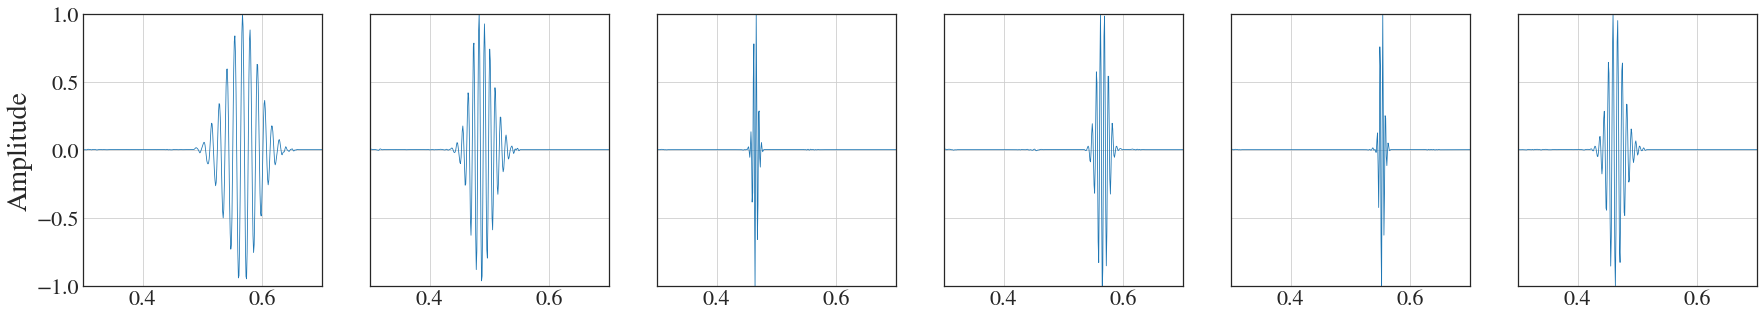
\includegraphics[width=\textwidth]{figures/generations/sg.png}
    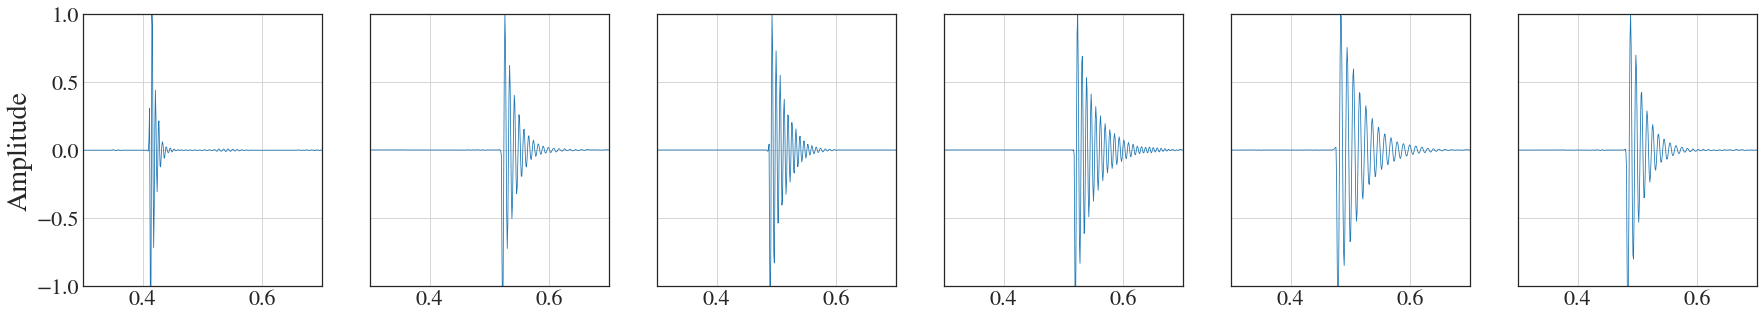
\includegraphics[width=\textwidth]{figures/generations/rd.png}
    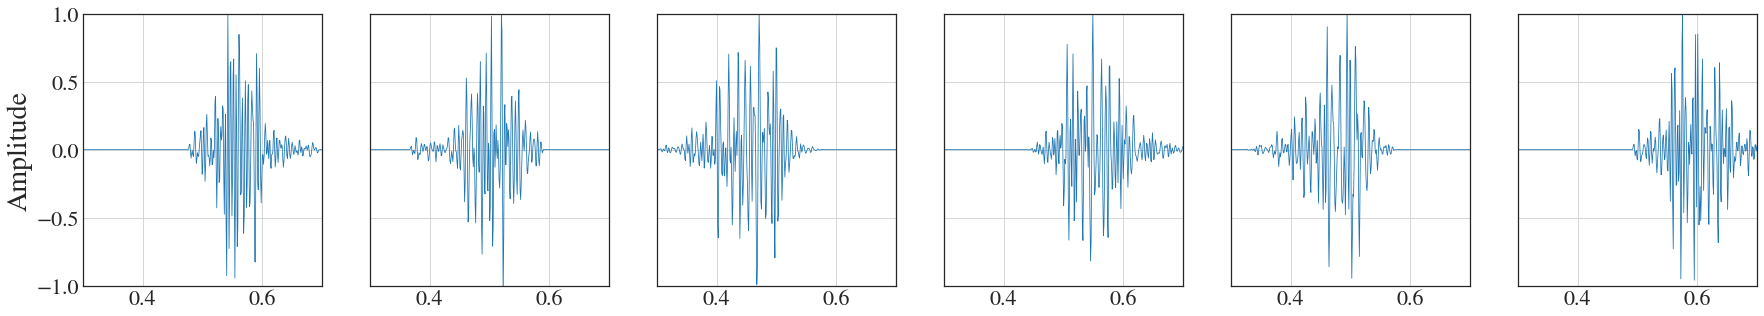
\includegraphics[width=\textwidth]{figures/generations/wnb.png}
    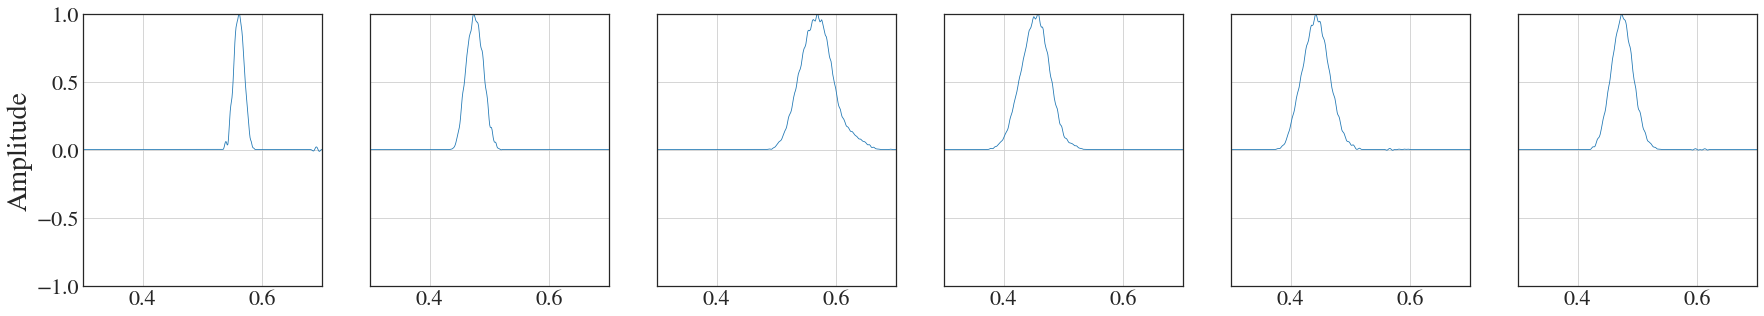
\includegraphics[width=\textwidth]{figures/generations/blip.png}
    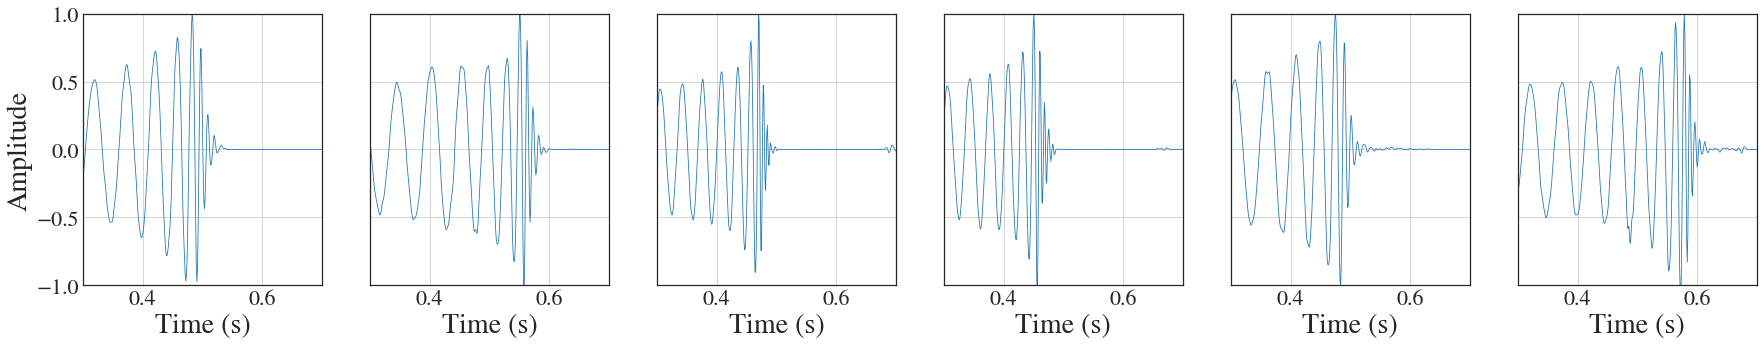
\includegraphics[width=\textwidth]{figures/generations/bbh.png}
    \caption{Examples of \ac{GW} burst signals generated by a conditional generative adversarial network. By row: Sine-Gaussian, Ringdown,
White-noise burst, Gaussian pulse, Binary black hole merger.}
\label{fig:gen_signals} \end{figure}

\subsection{Signal generation}
The generator network is a function G : $\mathbf{z},\mathbf{c} $ $\in$ $\mathbb{R}^{100}$ $\to$ $\mathbb{R}^{1024\times2}$, where $\mathbf{z},\mathbf{c}$ are the latent vector and class vector. Given a latent vector randomly sampled from a normal distribution with zero mean and unit variance, a class label which is represented by a 5 dimensional one-hot encoded vector for each class, the results from the generator can be seen in \cref{fig:gen_signals}. Each plot shows the output of the generator after given randomised $\mathbf{z}$ and one of the five class vectors $\mathbf{c}$.
 %Depending on the orientation of the detector with respect to a hypothetical signal in the sky, the waveforms may appear inverted, shifted in time and their strain attenuated. 

\subsection{Interpolation}
Machine learning algorithms are often described as universal function approximators. In the generators case it maps samples drawn from a 100 dimensional Gaussian space to its representation of the training set. As with any function, there should be a one to one mapping from the domain and co-domain to allow for smooth transitions across the latent space. One advantage of using GANs as a waveform generator is that once it is trained, it can perform rapid generations faster than computationally
expensive algorithms \michael{e.g.?}. For complicated data sets, the network architecture must be diverse and dense enough to capture distinct variations from the training set. Most GANs perform well on relatively low resolution image generations, however, higher resolutions demand larger networks and long training times. GANs attempting to replicate complicated structures and do not have the necessary architecture either struggle to produce results at all or fall into the common failure mode know as mode collapse; where the generator produces a small variety of samples or simply memorises the training set. To test this, we perform linear interpolations in the latent and class space. 

In this section we explore the latent space formed by the generator by interpolation. We take two random points in the latent space and linearly interpolate between them. These new latent space vectors can now be fed into the generator to make predictions on while keeping the class vectors constant. The full effect shown in \cref{fig:z_interp}. We can see that each plot shows plausible waveforms suggesting that the generator has constructed a smooth space unlike the discrete training case. Additionally as each class is given the same latent points to interpolate over, we can see that the waveforms cluster together with respect to their parameters. Visually, the sine-gaussian and ring-down waveforms share similar frequencies and the other signals show similar decays and starting epochs. The only exception is BBH waveforms, which is expected as they were trained with more variety of parameters and consistently have their peaks in the last quarter of the time series.

\begin{figure}
    \centering
    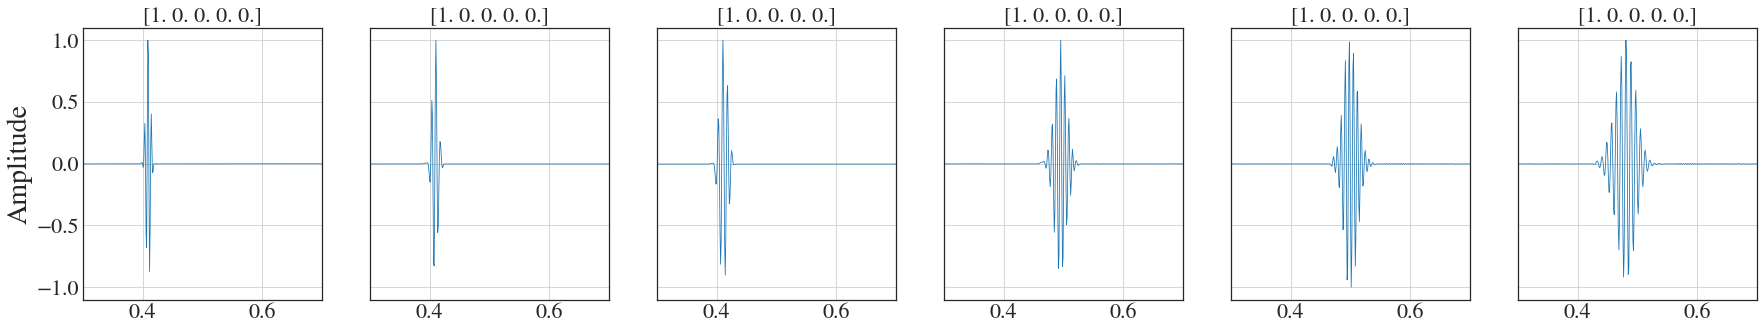
\includegraphics[width=\textwidth]{figures/generations/z_interp_sg.png}
    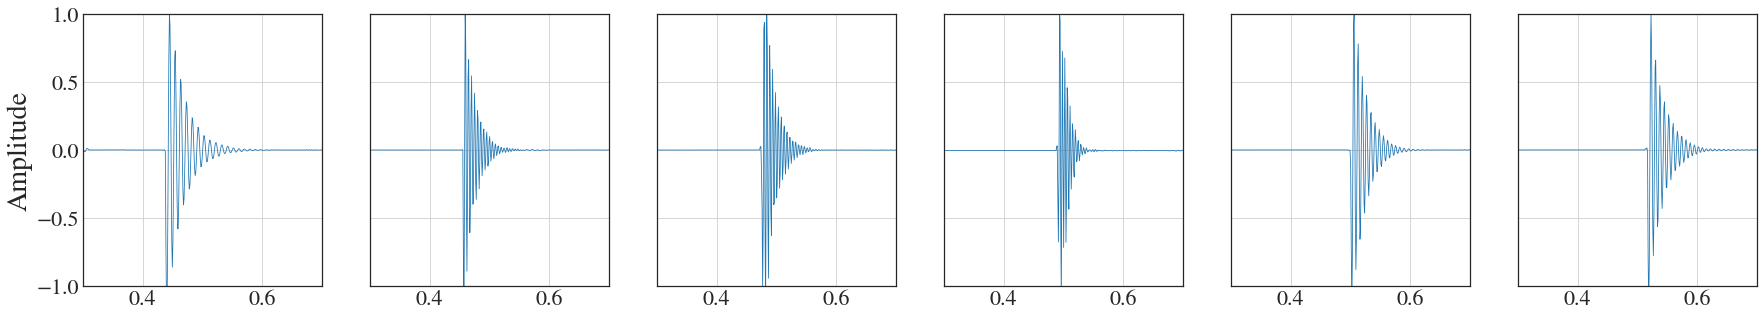
\includegraphics[width=\textwidth]{figures/generations/z_interp_rd.png}
    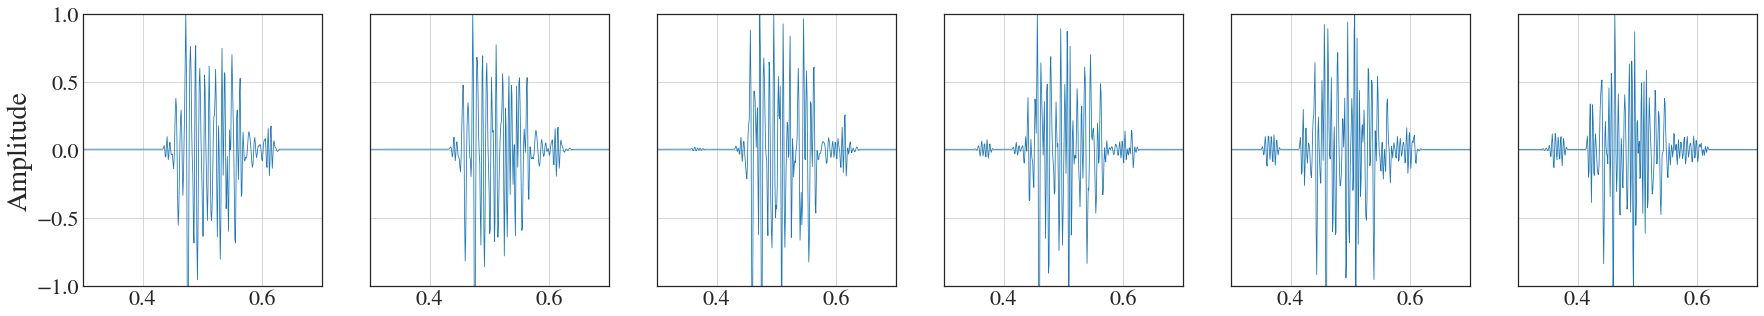
\includegraphics[width=\textwidth]{figures/generations/z_interp_wnb.png}
    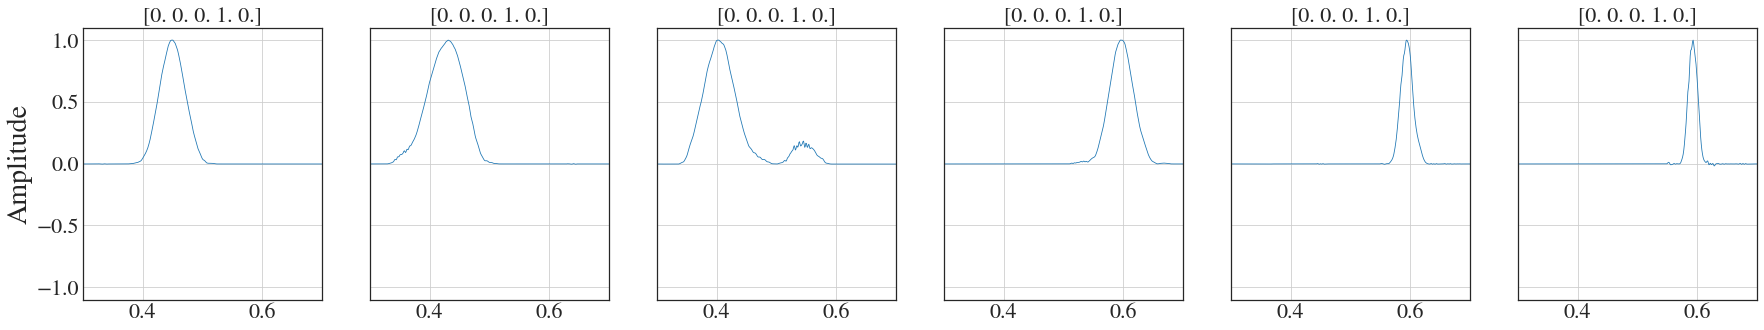
\includegraphics[width=\textwidth]{figures/generations/z_interp_blip.png}
    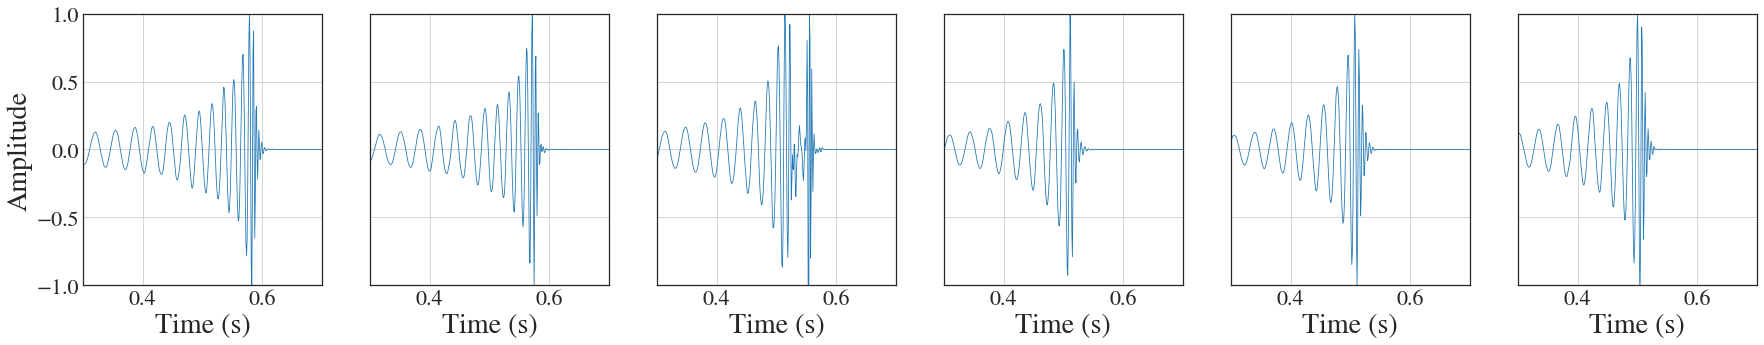
\includegraphics[width=\textwidth]{figures/generations/z_interp_bbh.png}
    \caption{Latent space linear interpolation, class space is constant.}
    \label{fig:z_interp}
\end{figure}

\subsubsection{Class space interpolation}
In order to explore the class space we keep the latent vector constant and interpolate through the 5 classes. We construct a path between the 5 waveforms and show that the space is populated enough to allow for transitions between classes. Sine-Gaussian to ringdown performs well in interpolation with each signal being a plausible burst GW. It is obvious that the GAN has clustered these two groups during training as they share many characteristics. The other signals have sharper transitions but still retain plausible looking waveforms. 

\begin{figure}
    \centering
    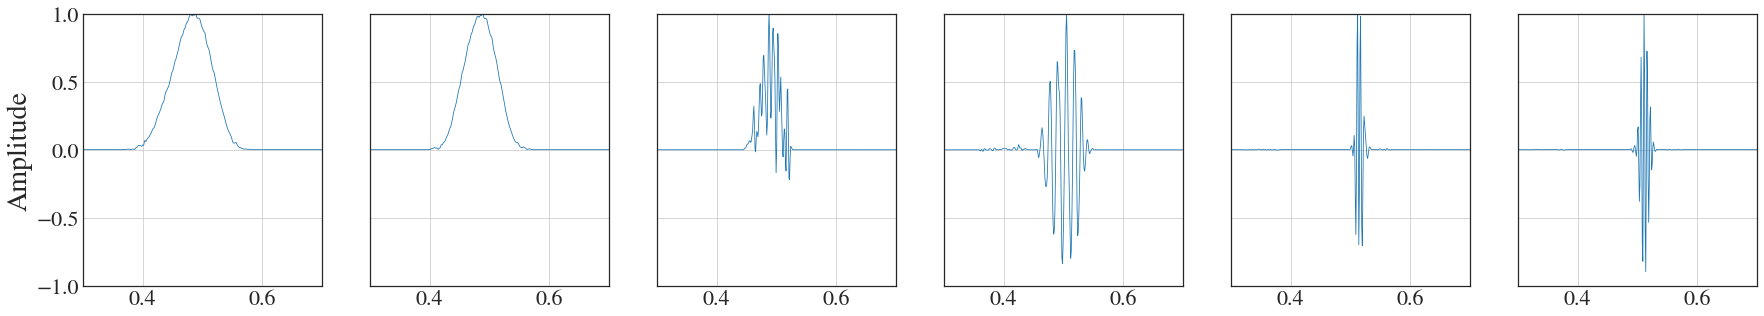
\includegraphics[width=\textwidth]{figures/generations/interp_blip-sg.png}
    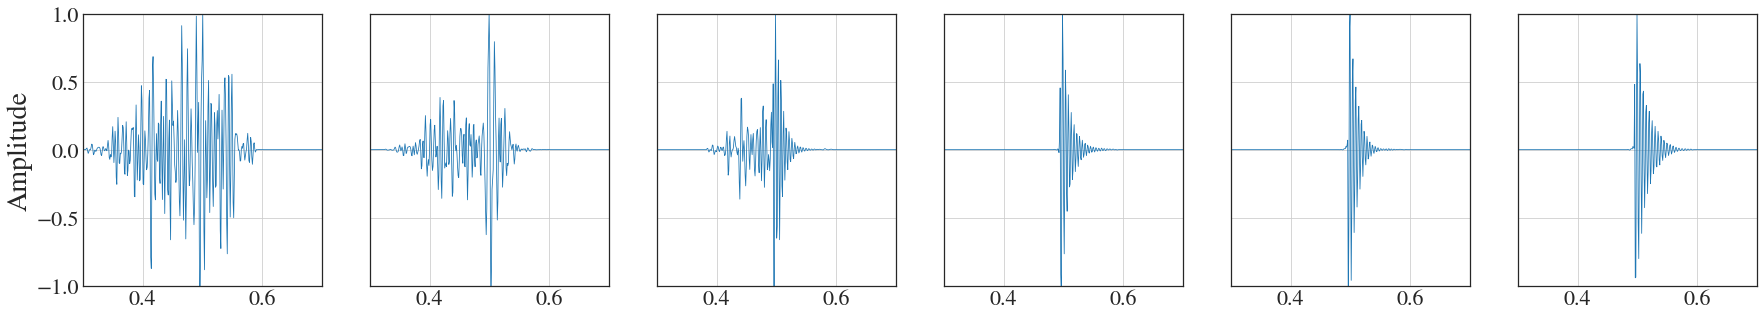
\includegraphics[width=\textwidth]{figures/generations/interp_wnb-rd.png}
    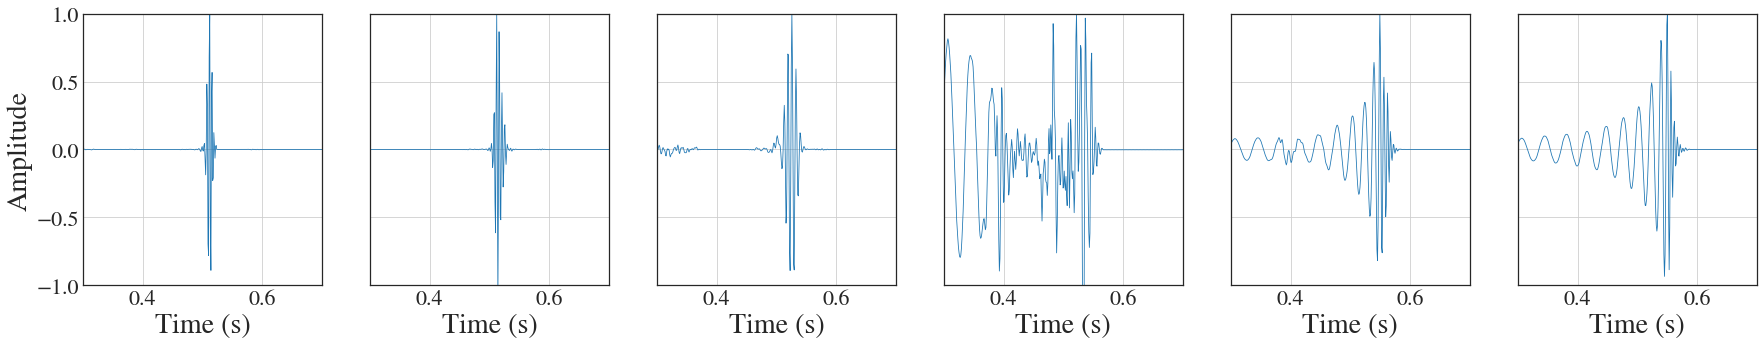
\includegraphics[width=\textwidth]{figures/generations/interp_sg-bbh.png}
    \caption{Class space linear interpolation, class space is held constant. Top row: gaussian blip to sine-gaussian, middle row: white noise burst to ringdown, bottom row: sine-gaussian to BBH.}
    \label{fig:c_interp}
\end{figure}

\subsection{Using a GAN to generate unmodelled waveforms}
So far the analysis has focused on interpolating between two classes of signals with the aim to use the interpolated signals as unmodelled waveforms, instead, we may consider random mixtures of classes. We defined the classes in one-hot encoding framework, that is, each class resides at the corner points of a 5 dimensional cube. In order to generate an even mixture of classes we sample points uniformly in this space. \jordan{this would be the box}. Alternativly we can sampe points from the plane that intersects the four corners, which for a 5-dimensional case is, sample from a 4-simplex. Thks can nbee seen in \ref{fig:unmodelled_samples}. \jordan{why? this enforces the vector points to sum to one. Why is that good? Well it keeps the points lying on the simplex.} 


\begin{figure}
    \centering
    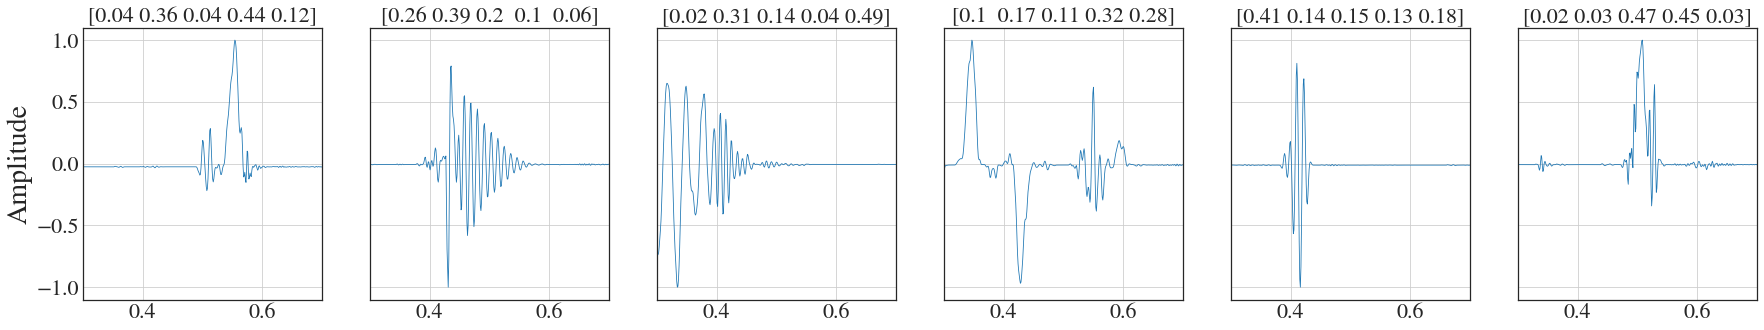
\includegraphics[width=\textwidth]{figures/generations/simplex_sample1.png}
    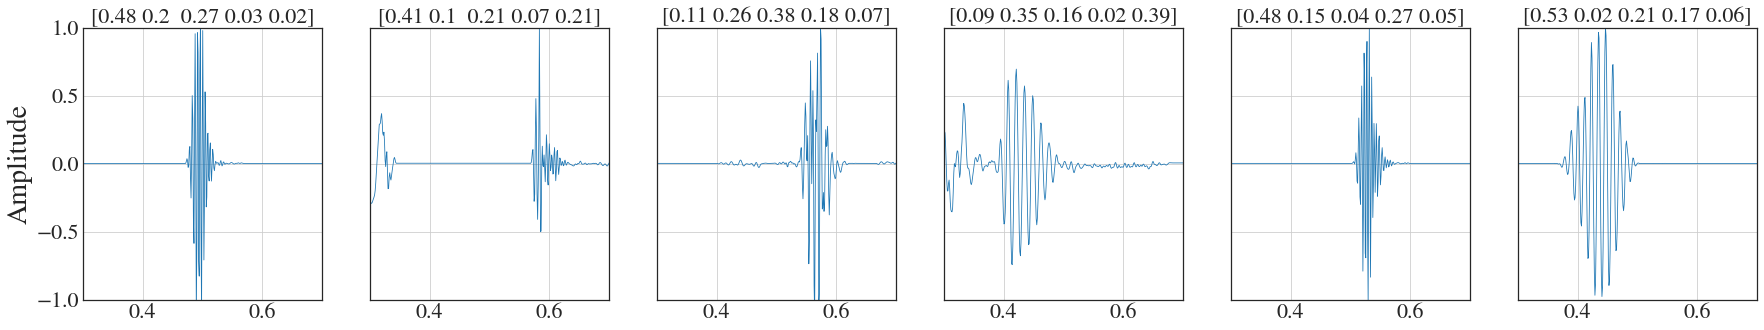
\includegraphics[width=\textwidth]{figures/generations/simplex_sample2.png}
    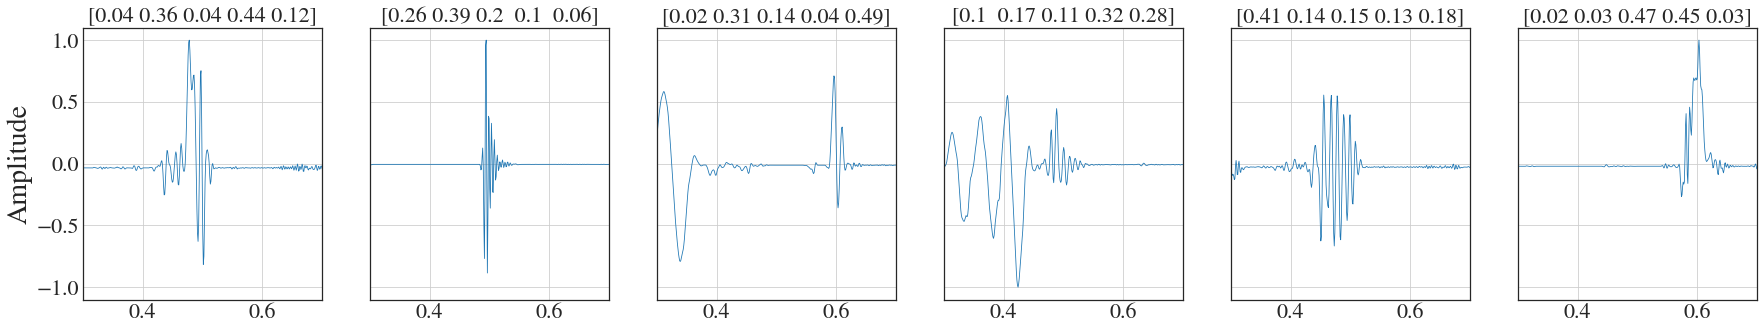
\includegraphics[width=\textwidth]{figures/generations/simplex_sample3.png}

    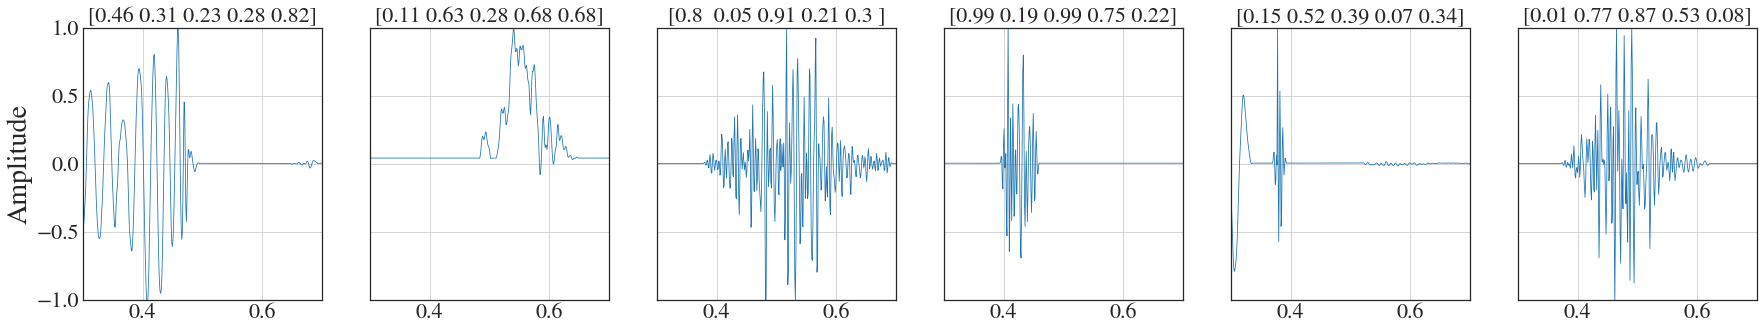
\includegraphics[width=\textwidth]{figures/generations/uniform_sample3.png}
    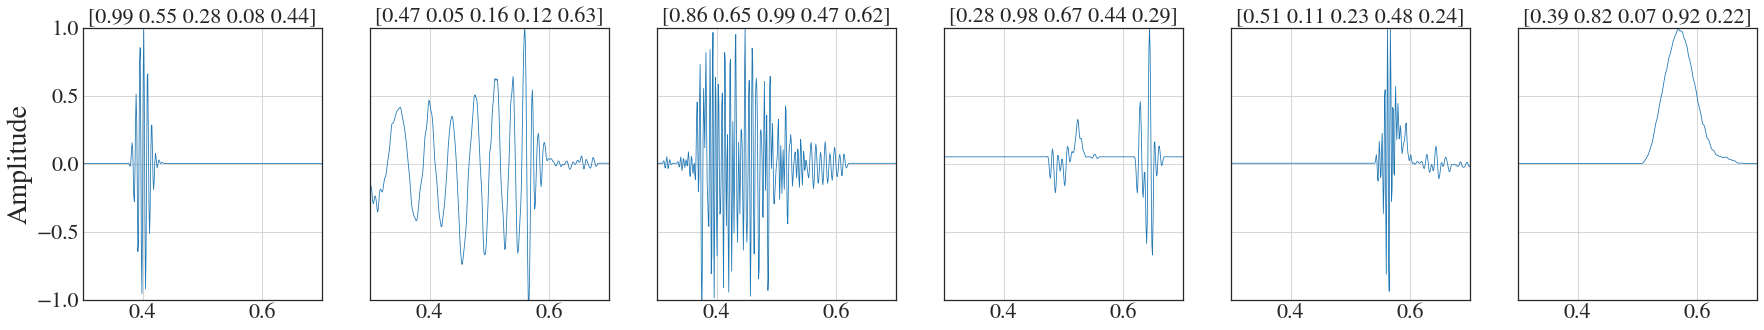
\includegraphics[width=\textwidth]{figures/generations/uniform_sample2.png}
    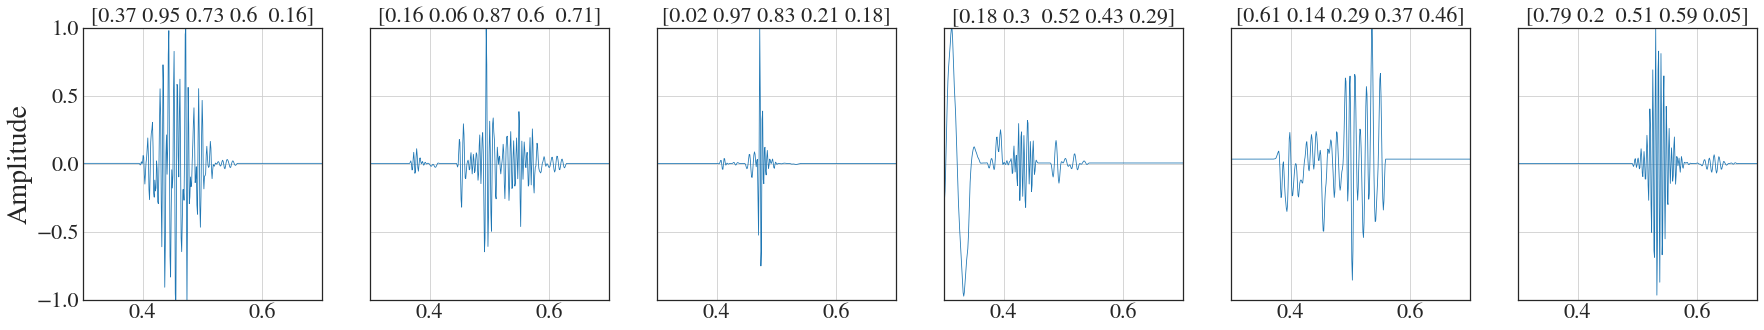
\includegraphics[width=\textwidth]{figures/generations/uniform_sample1.png}
    \caption{GAN generations where the class vectors are sampled from the 4-D plane and sampled uniformly in the class space.}
    \label{fig:unmodelled_samples}
\end{figure}


\begin{comment}
We can now think of ways to properly sample from the space between these points in a uniform way. Uniformity enforces the condition that we have a variety of waveforms. Thge easiest being to uniformly sample points in this space and use them as the class vectors for the generator. Another way would be to keep the magnitude of the class vector as 1. For a 5-dimensional space we would sample from the 4-dimensional plane that intersects the corner points. 
\end{comment}

\michael{We don't show any results with two detectors yet we use two detectors for the CNN, we might want to think when/where it's best to show some generations with both detectors. Maybe when we show a signal with noise since it's all part of the post-processing?}

\subsection{CNN analysis}
In this section of the analysis we will forensically compare generations from the GAN to help determine the success and failures of the model. We investigate a simple case of using a CNN to detect whether a signal is contained in noise or if the data is noise only. The signals we train the CNN on are generated from the GAN with their latent input randomised from a 100-dimensional Gaussian distribution and are categorised by their method of defining their class vector: 
\begin{itemize}
	\item Conditional – Definite categorical generations from the GAN. These signals are the closest to the training set.
	\item Uniform – Generated using a uniform distribution U[0,1] as the input class vector.
	\item Simplex – Generated using a Dirichlet distribution that samples from the 4-simplex as the input class vector. 
\end{itemize}
The CNN is trained to distinguish between two classes: signals in additive Gaussian noise and Gaussian noise, where “signals” are taken from either the Conditional, Uniform or Simplex cases. This means in total there are three CNNs to train and all CNNs share the same architectural structure. All of the training data used is “whitened” by a power spectral density (PSD) at Advanced LIGO design sensitivity, such that, there is equal power at each frequency and is correctly normalised. This procedure is applied to signals whose signal-to-noise ratios (SNRs) are defined prior to be in the range uniformly [1-16]. For each run the training data consists of 200,000 signals which contain one half noise only and one half signal contained in noise. Of that 80\% is used for training and 20\% used for validation. A different testing set is also used in analysis that is 200,000 in size. 

*table of parameters used for CNN*

In Fig. \ref{fig:roc_curves} we compare the CNN results between the three datasets, we train three CNNs on the Conditional, simplex and uniform data sets and use these models to make predictions on the other unseen datasets. We make a comparison by fixing the fraction of samples incorrectly identified as signals (false alarm rate) and plotting this versus the optimal SNR of the signals. 

\begin{figure}
    \centering
    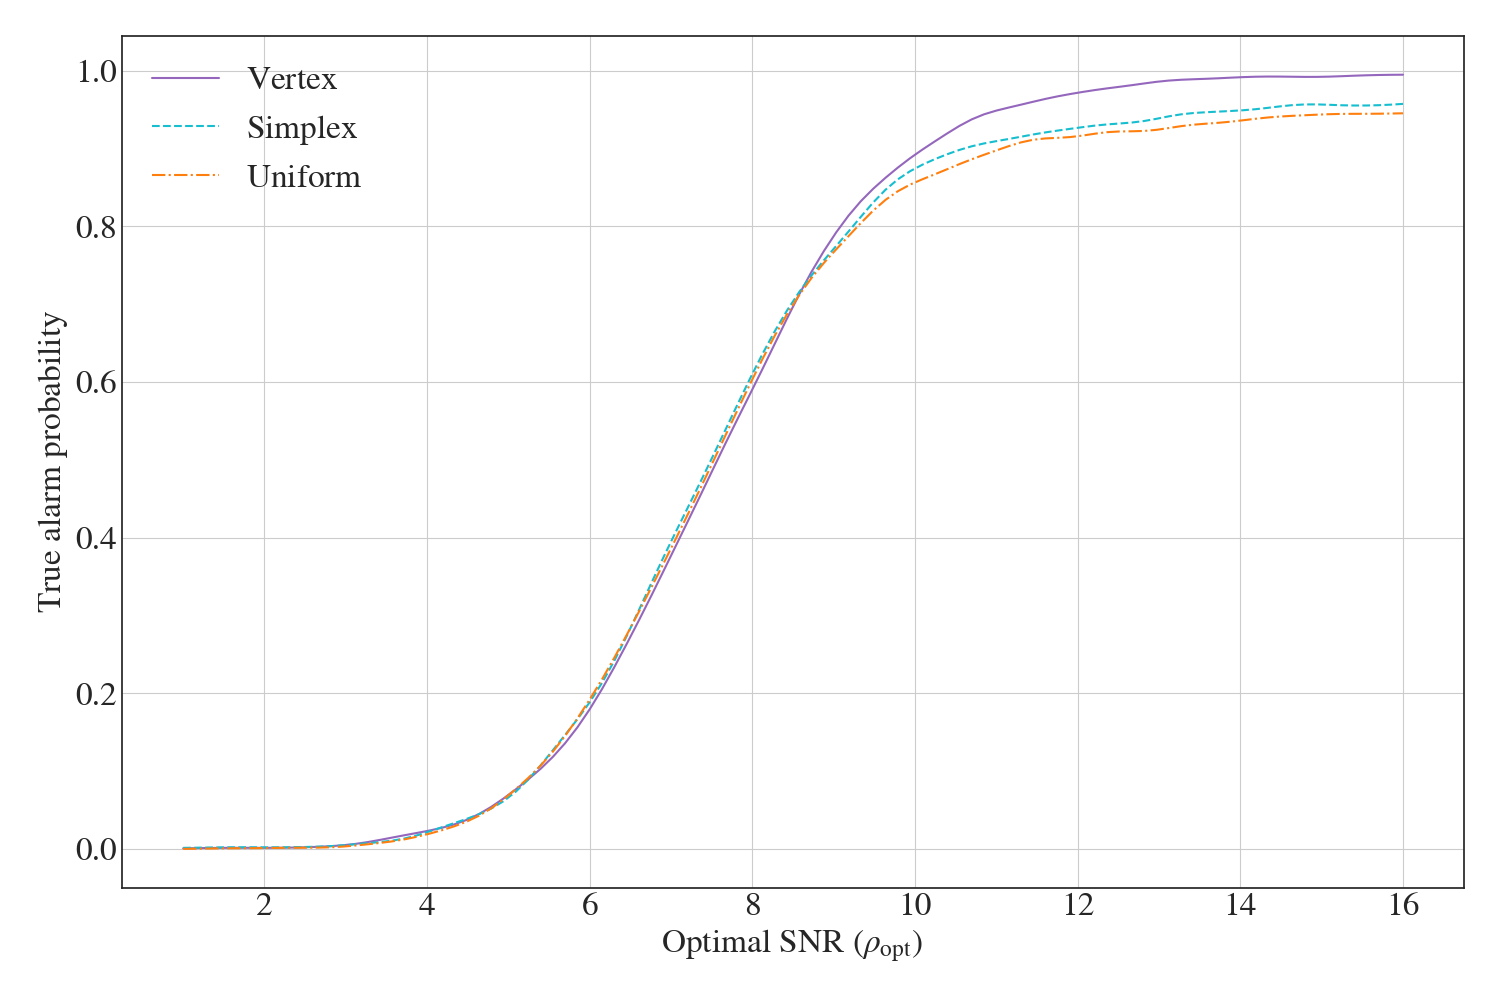
\includegraphics[width=0.8\textwidth]{figures/conditional_trained.png}
    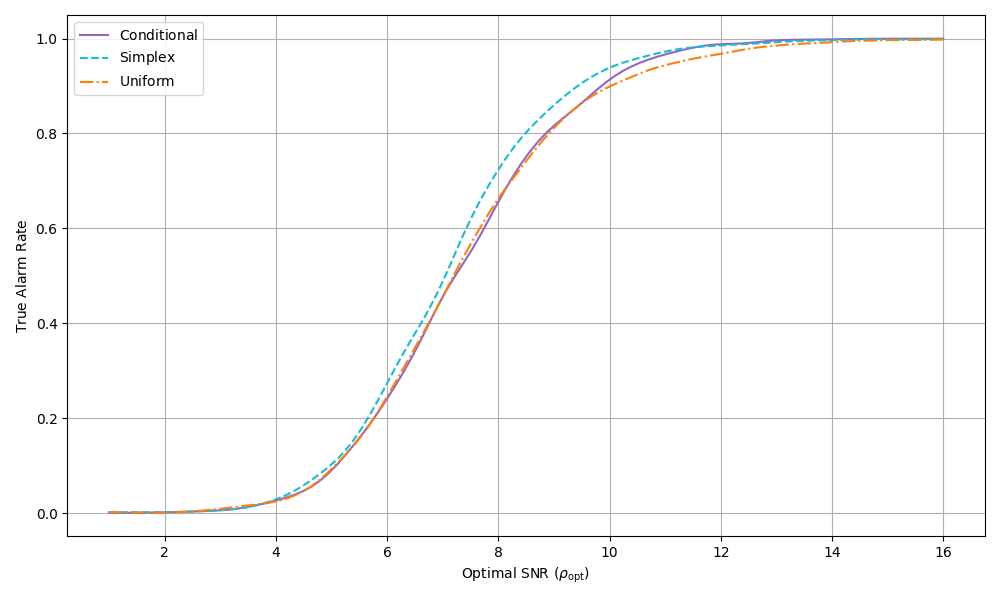
\includegraphics[width=0.8\textwidth]{figures/simplex_trained.png}
    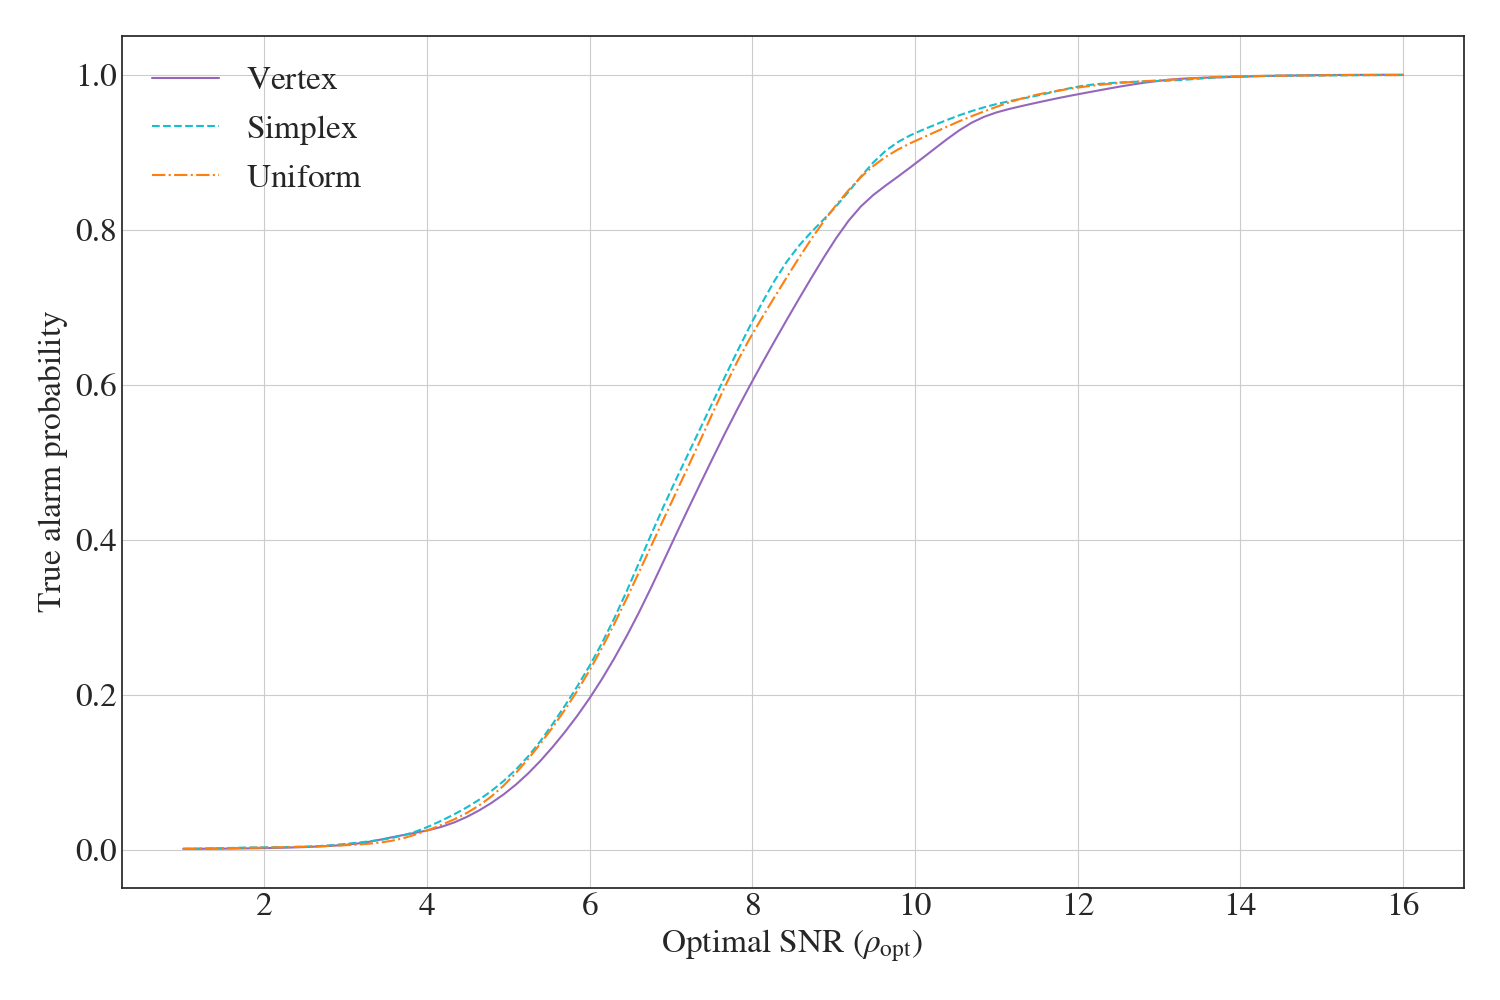
\includegraphics[width=0.8\textwidth]{figures/uniform_trained.png}

    \caption{Efficiency curves comparing the performance of CNNs trained on conditional generations (top), simplex generations (middle), uniform generations (bottom) for a fixed false alarm rate of $10^{-3}$.}
    \label{fig:roc_curves}
\end{figure}

These results show for a CNN trained on conditional signals, the uniform data set is distinguishable from the conditional and simplex dataset. The CNN is robust enough to capture the differences between the datasets and shows that the GAN can generate a variety of unmodelled waveforms that can be used in future testing. 

\begin{comment}
{\subsection{Vector Arithmetic}
In DCGANs the authors demonstrated unsupervised vector arithmetic with celebrity face generation. They kept points in the latent space and performed simple vector arithmetic to generate new images. This allows for intuitive and targeted generation of images. However, the authors realised that single images vectors were unstable and there was a need to average three vectors before any arithmetic. DCGANs is unconditional, therefore, the vectors used were chosen empirically, generating many faces and choosing the attributes for study. Here, we show that this GAN only needs a single vector representation and due to conditioning we can have more control over which vectors to use in the arithmetic. In \cref{fig:arithmetic} we generate a whitenoise burst and a BBH insprial using their respective class labels and use a randomised latent point and response. Keeping the latent point and response, we average the two class vectors and use this as input to the generator. \Cref{fig:arithmetic} (c) shows the generation based on the combined class vectors which visually looks similar to a supernova waveform. Supernova waveform generations require expensive numerical relativity simulations and various assumptions about the collapse of its parent star. Here, we are able to produce similar waves at a fraction of the expense and we are able to further modify the resultant by using different latent space samples. \jordan{this is the adding noise thing but i need to work out the correct way to do it with the directional vector}. 
\end{comment}



%%%%%%%%%%%%%%%%%%%%%%%%%%%%%%%%%%%%%%%%%%%%%%%%%%%%%%%%%%%%%%%%%%%%%%%%%%%%%%
\section{Conclusions}
%%%%%%%%%%%%%%%%%%%%%%%%%%%%%%%%%%%%%%%%%%%%%%%%%%%%%%%%%%%%%%%%%%%%%%%%%%%%%%
In this work we present the potential of Generative Adversarial Networks for burst ac{GW} analysis. We have shown that GANs have the ability to generate 5 class varieties of modelled burst \ac{GW} signals that can be generated at whim. The latent and class spaces were explored through interpolation and suggest that the space provides smooth translations between classes and overall waveform shape. We then showed targeted waveform generation by mixing classes to produce new unmodlled waveform varieties that can be used to test current burst search pipelines. \jordan{couple of sentences about classifier}. 

In order to extend this work to a viable burst wave generator and classifier a few points require further research. In principle it is trivial to add another detector inside the response layer \jordan{response is the wrong thing to say since the time delay isnt really a response, extrinsic layer? just non trainable layer? The box?}, however, as this now 3 dimensional signal is feed to the discriminator this will no doubt require further tweaking of the network. We can add more burst-like wave forms in the training set, like detector glitches which would similarly require further network design. The work presented here is noise free. To havea complete generation and detection package we would like to train the network on signals hidden in additive Gaussian noise and test the ability of the auxiliary classifier. 

The approach shown in this work shows promise in generating unmodelled burst waveforms from exotic sources. Having the ability to quickly generate new waveforms is essential to test current detection schemes and their susceptibilty to unmodelled sources. We belive that GANs have the ability to generate high fidelity waveforms at a fraction of the computational expense and do not rely on large prior parameter space. Having banks of these waveforms at hand can aid in our understand of the physics processes behind these non-standard ac{GW} emitters.  

\jordan{I want to include a link to the github etc but also a google collab scrip like the one for BigGANs: \\
\url{https://colab.research.google.com/github/tensorflow/hub/blob/master/examples/colab/biggan_generation_with_tf_hub.ipynb.} 
It's fun and gives a better feel for the interpolating that static images.}

\begin{comment}
\begin{itemize}
\item Summarise the paper
\item Dedicate a paragraph to each of the key results discussed in the previous
section
\item Have at least one paragraph on the future directions of this work
\item Conclude with a positive paragrpah about the potential uses and impact of
the approach.
\end{itemize}
\end{comment}

\section*{References}
\bibliography{references}

\clearpage

\appendix
\section{List of hyperparameters}
\begin{table}[hb]
\caption{CGAN architecture}
\footnotesize
\begin{tabular}{@{}l l l l l l l}
\br
 Operation & Kernel & Strides & Output Shape & BN & Dropout & Activation \\
\mr
 G(\textbf{z}): Input \textbf{z} $\sim$ Normal(0,0.02) & N/A & N/A & (100,) & \ding{55} & 0 & N/A \\  
 Dense & N/A & N/A & (32768,) & \ding{55} & 0 & ReLU \\  
 Class input c & N/A & N/A & (1,) & \ding{55} & 0 & N/A \\
 Embedding & N/A & N/A & (1, 120) & \ding{55} & 0 & N/A \\
 Dense & N/A & N/A & (1,128) & \ding{55} & 0 & ReLU \\ 
 Reshape \textbf{z} & N/A & N/A & (128, 256) & \ding{55} & 0 & N/A \\
 Reshape c & N/A & N/A & (128, 1) & \ding{55} & 0 & N/A \\
 Concatenate & N/A & N/A & (128, 257) & \ding{55} & 0 & N/A \\
 Reshape & N/A & N/A & (64, 514) & \ding{55} & 0 & N/A \\
 Transposed Convolution & 18x1 & 2 & (256, 256) & \ding{51} & 0 & ReLU\\
 Transposed Convolution & 18x1 & 2 & (512, 128) & \ding{55} & 0 & ReLU\\
 Transposed Convolution & 18x1 & 2 & (1024, 64) & \ding{55} & 0 & ReLU\\
 Convolution & 18x1 & 1 & (1024, 1) & \ding{55} & 0 & Tanh \\
 Sky input & N/A & N/A & (3,) & \ding{55} & 0 & N/A \\
 Concatenate & N/A & N/A & (1027,) &  \ding{55} & 0 & N/A \\
 Lambda & N/A & N/A & (1024, 2) & \ding{55} & 0 & N/A \\
 D(\textbf{x}): Input \textbf{x} & N/A & N/A & (1024, 2) & \ding{55} & 0 & N/A \\
 Convolution & 14x1 & 2 & (512, 64) & \ding{55} & 0.5 & Leaky ReLU \\
 Convolution & 14x1 & 2 & (256, 128) & \ding{55} & 0.5 & Leaky ReLU \\
 Convolution & 14x1 & 2 & (128, 256) & \ding{55} & 0.5 & Leaky ReLU \\
 Convolution & 14x1 & 2 & (64, 512) & \ding{55} & 0.5 & Leaky ReLU \\
 Flatten & N/A & N/A & (32768,) & \ding{55} & 0 & N/A \\
 Dense & N/A & N/A & (1,) & \ding{55} & 0 & Sigmoid \\
 Dense & N/A & N/A & (5,) & \ding{55} & 0 & Softmax \\
\br
 Optimizer & \multicolumn{6}{l}{Adam($\alpha$ = 0.0002, $\beta_{1}$ = 0.5)} \\
 Batch size & \multicolumn{6}{l}{128}  \\
 Iterations & \multicolumn{6}{l}{60000}  \\
 Leaky ReLU slope & \multicolumn{6}{l}{0.2} \\
 Weight initialization & \multicolumn{6}{l}{Gaussian($\mu$ = 0, $\sigma$ = 0.02)} \\
 Generator loss & \multicolumn{6}{l}{Binary cross-entropy} \\
 Discriminator loss & \multicolumn{6}{l}{Binary cross-entropy \& sparse categorical cross-entropy} \\ 
 \br
\end{tabular}\\
\label{Tab:hyperparameters}
\end{table}
\normalsize

\section{Many more generated examples}

\end{document}

